
\chapter{拟凝聚层的\trCech{}上同调}
\label{ch:cech-cohomology}

这个主题出人意料地简单而优美。你或许会觉得\trCohomology{}必定复杂，而这也正是它出现得如此靠后的原因。但你将会看到，我们需要的背景极少。在定义\trScheme{}之后，我们本可以立刻定义\trQCSheaf，接着定义\trCohomology，并验证它具有许多有用的性质。


\section{上同调的（理想）性质}

我们并不立刻定义\trQCSheaf{}的\trCohomology，而是先讨论我们为何关心它，以及它应当具有哪些性质。

由于 $\Gamma(X,\cdot)$ 是一个\trLeftExact{}函子，若
$0\to\mathscr{F}\to\mathscr{G}\to\mathscr{H}\to 0$ 是概形 $X$ 上诸\trQCSheaf{}的一个\trShortExactSequence，则
\[
0\longrightarrow \mathscr{F}(X)\longrightarrow \mathscr{G}(X)\longrightarrow \mathscr{H}(X)
\]
是正合的。我们梦想这个序列能向右延续下去，给出一个\trLongExactSequence。更明确地说：应当存在一些协变函子
$\mathrm{H}^i$（$i\ge 0$），把 $X$ 上的\trQCSheaf{}送到\trGroup，使得 $\mathrm{H}^0$ 就是\trGlobalSections{}函子
$\Gamma$，并且有「上同调中的\trLongExactSequence」。
\begin{equation*}\tag{18.1.0.1}\label{eq:cohomology-long-exact-seq}
\begin{gathered}
0\longrightarrow \mathrm{H}^0(X,\mathscr{F})\longrightarrow \mathrm{H}^0(X,\mathscr{G})\longrightarrow \mathrm{H}^0(X,\mathscr{H})\\[10pt]
\longrightarrow \mathrm{H}^1(X,\mathscr{F})\longrightarrow \mathrm{H}^1(X,\mathscr{G})\longrightarrow \mathrm{H}^1(X,\mathscr{H})\longrightarrow\cdots
\end{gathered}
\end{equation*}

（一般地，每当我们见到一个\trLeftExact{}或\trRightExact{}的函子，都应当盼望这件事；而在好的情形里，我们的梦想将会成真。这背后的机关通常涉及\emph{\trDerivedFunctor}（derived functor），我们将在第 23 章讨论。）

在显式定义\trQCSheaf{}的各\trCohomology{}群之前，我们先描述它们的重要性质；这些性质在某些方面甚至比形式定义还要重要。加了框的性质才是重要的。

设 $X$ 是一个\emph{分离且拟紧}的 $A$-\trScheme。对 $X$ 上每个\trQCSheaf{} $\mathscr{F}$，我们都将定义 $A$-\trModule{}
$\mathrm{H}^i(X,\mathscr{F})$。特别地，若 $A=k$，它们就是 $k$-\trVectorSpace；此时我们定义
$h^i(X,\mathscr{F})=\dim_k\mathrm{H}^i(X,\mathscr{F})$（在左边，$k$ 被隐去不写）。

\textbf{(i)}\quad 每个 \fbox{$\mathrm{H}^i$ 都是从 $\mathit{QCoh}_X$ 到 $\mathit{Mod}_A$ 的协变函子}。

\textbf{(ii)}\quad 函子 $\mathrm{H}^0$ 被等同于函子 $\Gamma$：\fbox{$\mathrm{H}^0(X,\mathscr{F})=\Gamma(X,\mathscr{F})$，}而且 \textbf{(i)} 的协变性在 $i=0$ 时不过是 $\Gamma$ 的寻常协变性（$\mathscr{F}\to\mathscr{G}$ 诱导
$\Gamma(X,\mathscr{F})\to\Gamma(X,\mathscr{G})$）。

\textbf{(iii)}\quad 若 $0\to\mathscr{F}\to\mathscr{G}\to\mathscr{H}\to 0$ 是 $X$ 上诸\trQCSheaf{}的一个\trShortExactSequence，则我们有一条 \fbox{\trLongExactSequence}（\eqref{eq:cohomology-long-exact-seq}）。映射
$\mathrm{H}^i(X,\mathscr{F})\to\mathrm{H}^i(X,\mathscr{G})$ 来自协变性，
$\mathrm{H}^i(X,\mathscr{G})\to\mathrm{H}^i(X,\mathscr{H})$ 亦然；至于\emph{\trConnectingHomomorphism}（connecting homomorphism）
$\mathrm{H}^i(X,\mathscr{H})\to\mathrm{H}^{i+1}(X,\mathscr{F})$，则尚有待定义。

\textbf{(iv)}\quad 若 $\pi\colon X\to Y$ 是拟紧分离 $A$-\trScheme{}之间的任意一个\trMorphism，而 $\mathscr{F}$ 是 $X$ 上的一个\trQCSheaf，则存在自然的\trMorphism{}
\fbox{$\mathrm{H}^i(Y,\pi_*\mathscr{F})\to\mathrm{H}^i(X,\mathscr{F})$}，它是
$\Gamma(Y,\pi_*\mathscr{F})\to\Gamma(X,\mathscr{F})$ 的扩张。（注意：由关于拟紧与分离态射的\trCancellationTheorem{}~11.1.1——在该定理的陈述中取 $Z=\Spec A$——$\pi$ 确实既拟紧又分离，于是由\mbox{练习~14.4.C}，$\pi_*\mathscr{F}$ 确实是\trQCSheaf。）我们日后会看到，这是一个更大故事——\emph{\trLeray\trSpectralSequence}（\mbox{定理~23.4.5}）——的一部分。若 $\mathscr{G}$ 是 $Y$ 上的一个\trQCSheaf，则令 $\mathscr{F}:=\pi^*\mathscr{G}$，并利用伴随映射
$\mathscr{G}\to\pi_*\pi^*\mathscr{G}$ 与协变性（性质 (i)），便得到一个自然的\textbf{\trPullback{}映射}（pullback map）
$\mathrm{H}^i(Y,\mathscr{G})\to\mathrm{H}^i(X,\pi^*\mathscr{G})$（经由
$\mathrm{H}^i(Y,\mathscr{G})\to\mathrm{H}^i(Y,\pi_*\pi^*\mathscr{G})\to\mathrm{H}^i(X,\pi^*\mathscr{G})$），它是
$\Gamma(Y,\mathscr{G})\to\Gamma(X,\pi^*\mathscr{G})$ 的扩张。如此一来，$\mathrm{H}^i$ 便是「在空间上的\trContravariantFunctor」。

\textbf{(v)}\quad 若 $\pi\colon X\to Y$ 是一个\trAffine\trMorphism，而 $\mathscr{F}$ 是 $X$ 上的一个\trQCSheaf，则 \textbf{(iv)} 中的自然映射是一个\trIsomorphism：\fbox{$\mathrm{H}^i(Y,\pi_*\mathscr{F})\overset{\sim}{\longrightarrow}\mathrm{H}^i(X,\mathscr{F})$.}当 $\pi$ 是\trClosedEmbedding{}而 $Y=\mathbb{P}^N_A$ 时，这个\trIsomorphism{}把任意\trProjective{} $A$-\trScheme{}上的计算转译为 $\mathbb{P}^N_A$ 上的计算。

\textbf{(vi)}\quad（\emph{仿射覆盖上同调消失}，affine cover cohomology vanishing）若 $X$ 可以被 $n$ 个\trAffine{}开集覆盖，则对一切 $i\ge n$ 与一切 $\mathscr{F}$，
\fbox{$\mathrm{H}^i(X,\mathscr{F})=0$}。特别地，在\trAffine\trScheme{}上，一切更高次（$i>0$）的\trQC{}\trCohomology{}群都消失。此时 $\mathrm{H}^1$ 的消失，连同 \textbf{(iii)} 的\trLongExactSequence，蕴涵 $\Gamma$ 在\trAffine\trScheme{}的\trQCSheaf{}上是\trExact{}函子——这件事我们早已知道（\mbox{练习~6.3.A}）。

\textbf{18.1.1.}\ \emph{\trhRemark}（并非性质 \textbf{(vi)} 的一部分）。还有一条也是真的：若 $\dim X=n$，则对一切 $i>n$ 与一切 $\mathscr{F}$，
$\mathrm{H}^i(X,\mathscr{F})=0$（\textbf{维数上同调消失}，dimensional cohomology vanishing）。我们将对射影 $k$-\trScheme（\mbox{定理~18.2.6}）乃至拟射影 $k$-\trScheme（\mbox{练习~22.4.T}）证明这一点；一般情形的讨论见 \S18.2.7。

而当 $n=1$ 时，\textbf{(vi)} 的逆命题就是\trSerre{}的\emph{仿射性的上同调判别法}（cohomological criterion for affineness）；见 \S18.8.4。

我们回到清单上来吧。

\textbf{(vii)}\quad 函子 $\mathrm{H}^i$ 在\trDirectSum{}下表现良好，在\trFiltered\trColimit{}下亦然（此系更一般的情形）：\fbox{$\mathrm{H}^i(X,\colim\mathscr{F}_j)=\colim\mathrm{H}^i(X,\mathscr{F}_j)$.}

\textbf{(viii)}\quad 我们还将把 $\mathbb{P}^n_A$ 上所有 $\OO(m)$ 的\trCohomology{}辨识出来：

\textbf{18.1.2.\ \trhTheorem。}\ ——

（a）\emph{$\mathrm{H}^0(\mathbb{P}^n_A,\OO_{\mathbb{P}^n_A}(m))$ 是秩为 $\binom{n+m}{m}$ 的自由 $A$-\trModule，若 $m\ge 0$。}

（b）\emph{$\mathrm{H}^n(\mathbb{P}^n_A,\OO_{\mathbb{P}^n_A}(m))$ 是秩为 $\binom{-m-1}{-n-m-1}$ 的自由 $A$-\trModule，若 $m\le -n-1$。}

（c）\emph{$\mathrm{H}^i(\mathbb{P}^n_A,\OO_{\mathbb{P}^n_A}(m))=0$，其余情形。}

第一条陈述我们已在\mbox{重要练习~15.1.C}（另见 \S15.1.2）中证明过。我们在那里（又在\mbox{练习~15.1.D} 中）看到：把
$\mathrm{H}^0(\mathbb{P}^n_A,\OO_{\mathbb{P}^n_A}(m))$ 解释为 $A[x_0,\dots,x_n]$ 中 $m$ 次的\trHomogeneous{}多项式是大有好处的事。类似地，我们将会发现
$\mathrm{H}^n(\mathbb{P}^n_A,\OO_{\mathbb{P}^n_A}(m))$ 可以解释为
$(x_0x_1\cdots x_n)^{-1}A[x_0^{-1},\dots,x_n^{-1}]$ 中齐次次数为 $-m$ 的那些项（见\mbox{注记~18.3.5}）。

\mbox{定理~18.1.2} 有若干特征，它们将是我们日后所要证明的那些事实的首次登场：
\begin{itemize}[leftmargin=2.6em,itemsep=2pt,topsep=3pt]
\item 这些层的\trCohomology{}在高于 $n$ 的次数上消失（上文 \textbf{(vi)}，「仿射覆盖上同调消失」）。
\item 这些\trCohomology{}群总是\emph{有限生成}的 $A$-\trModule。这对\trProjective{} $A$-\trScheme{}上的所有\trCoherentSheaf{}都将会成立（\mbox{定理~18.1.3(i)}），而且（多费些功夫）对\trProper{} $A$-\trScheme{}也成立（\trGrothendieck{}凝聚定理~18.9.1）。
\item 最高次\trCohomology{}群在 $m>-n-1$ 时消失。我们日后会看到，这是\emph{\trKodaira{}消失}（Kodaira vanishing）的一个例子；见 \S21.5.7。
\end{itemize}

若 $A$ 是域 $k$：
\begin{itemize}[leftmargin=2.6em,itemsep=2pt,topsep=3pt]
\item 最高次\trCohomology{}群在 $m=-n-1$ 时是一维的。这是\emph{\trCanonical{}层}（canonical sheaf）或\emph{\trDualizingSheaf}（dualizing sheaf）的首次登场。
\item 存在一个自然的\trPerfectPairing
\[
\mathrm{H}^i(\mathbb{P}^n,\OO(m))\times\mathrm{H}^{n-i}(\mathbb{P}^n,\OO(-n-1-m))\longrightarrow\mathrm{H}^n(\mathbb{P}^n,\OO(-n-1)).
\]
这是\emph{\trSerreDuality}（Serre duality）的首次登场。（$n=1$ 的情形见\mbox{例~18.5.4}。）
\item 交错和 $\sum(-1)^i h^i(\mathbb{P}^n,\OO(m))$ 是 $m$ 的多项式。这是\emph{\trHilbert{}多项式}（Hilbert polynomial）的第一个例子。
\end{itemize}

在证明这些事实之前，让我们先用它们来证明一些有趣的东西，权作动机。由\mbox{定理~16.1.1}，对 $\mathbb{P}^n_A$ 上任意\trCoherentSheaf{} $\mathscr{F}$，我们都能找到一个满射
$\OO(m)^{\oplus j}\to\mathscr{F}$，由此得到正合列
\begin{equation*}\tag{18.1.2.1}\label{eq:coherent-sheaf-surjection}
0\longrightarrow \mathscr{G}\longrightarrow \OO(m)^{\oplus j}\longrightarrow \mathscr{F}\longrightarrow 0
\end{equation*}
其中 $\mathscr{G}$ 是某个\trCoherentSheaf。我们可以用它来证明下述结论。

\textbf{18.1.3.\ \trhTheorem。}\ ——\ \emph{(i) 对 $A$ 为\trNoetherian{}的\trProjective{} $A$-\trScheme{} $X$ 上的任意\trCoherentSheaf{} $\mathscr{F}$，$\mathrm{H}^i(X,\mathscr{F})$ 是一个凝聚（有限生成）的 $A$-\trModule。
(ii)（\trSerre{}消失）此外，当 $m\gg 0$ 时，对一切 $i>0$ 都有 $\mathrm{H}^i(X,\mathscr{F}(m))=0$。}

（\mbox{定理~18.7.F} 将给出一个稍稍更花哨的\trSerre{}消失版本。）

\emph{证明。}\quad 由于\trClosedSubscheme{}的\trCohomology{}可以在环绕空间上计算（上文 \textbf{(v)}），我们可以立即化归到 $X=\mathbb{P}^n_A$ 的情形。
(i) 考察长正合列：
\[
\begin{gathered}
0\longrightarrow \mathrm{H}^0(\mathbb{P}^n_A,\mathscr{G})\longrightarrow \mathrm{H}^0(\mathbb{P}^n_A,\OO(m)^{\oplus j})\longrightarrow \mathrm{H}^0(\mathbb{P}^n_A,\mathscr{F})\longrightarrow\\[10pt]
\mathrm{H}^1(\mathbb{P}^n_A,\mathscr{G})\longrightarrow \mathrm{H}^1(\mathbb{P}^n_A,\OO(m)^{\oplus j})\longrightarrow \mathrm{H}^1(\mathbb{P}^n_A,\mathscr{F})\longrightarrow\cdots\\[10pt]
\cdots\longrightarrow \mathrm{H}^{n-1}(\mathbb{P}^n_A,\mathscr{G})\longrightarrow \mathrm{H}^{n-1}(\mathbb{P}^n_A,\OO(m)^{\oplus j})\longrightarrow \mathrm{H}^{n-1}(\mathbb{P}^n_A,\mathscr{F})\longrightarrow\\[10pt]
\mathrm{H}^n(\mathbb{P}^n_A,\mathscr{G})\longrightarrow \mathrm{H}^n(\mathbb{P}^n_A,\OO(m)^{\oplus j})\longrightarrow \mathrm{H}^n(\mathbb{P}^n_A,\mathscr{F})\longrightarrow 0
\end{gathered}
\]
这个正合列到此终结，因为 $\mathbb{P}^n_A$ 被 $n+1$ 个\trAffine{}开集所覆盖（上文 \textbf{(vi)}，「仿射覆盖上同调消失」）。于是由\mbox{定理~18.1.2(b)} 与 \textbf{(vii)}，
$\mathrm{H}^n(\mathbb{P}^n_A,\OO(m)^{\oplus j})$ 是有限生成的，从而对\emph{一切}\trCoherentSheaf{} $\mathscr{F}$，
$\mathrm{H}^n(\mathbb{P}^n_A,\mathscr{F})$ 都是有限生成的。特别地，$\mathrm{H}^n(\mathbb{P}^n_A,\mathscr{G})$ 是有限生成的。既然
$\mathrm{H}^{n-1}(\mathbb{P}^n_A,\OO(m)^{\oplus j})$ 是有限生成的，而 $\mathrm{H}^n(\mathbb{P}^n_A,\mathscr{G})$ 亦然，我们便知道：对一切\trCoherentSheaf{} $\mathscr{F}$，
$\mathrm{H}^{n-1}(\mathbb{P}^n_A,\mathscr{F})$ 是有限生成的。我们继续向下归纳。
(ii) 将 \eqref{eq:coherent-sheaf-surjection} 用 $\OO(N)$ 扭转，其中 $N\gg 0$。那么
\[
\mathrm{H}^n(\mathbb{P}^n_A,\OO(m+N)^{\oplus j})=\mathrm{H}^n(\mathbb{P}^n_A,\OO(m+N))^{\oplus j}=0
\]
（由上文 \textbf{(vii)}），于是 $\mathrm{H}^n(\mathbb{P}^n_A,\mathscr{F}(N))=0$。翻译一下：对任何\trCoherentSheaf，只要你用 $\OO(N)$（$N$ 充分大）加以扭转，它的最高次\trCohomology{}便消失。所以这对 $\mathscr{G}$ 也成立。于是由\trLongExactSequence，当 $N\gg 0$ 时
$\mathrm{H}^{n-1}(\mathbb{P}^n_A,\mathscr{F}(N))=0$。与 (i) 一样，我们向下归纳，直到得到
$\mathrm{H}^1(\mathbb{P}^n_A,\mathscr{F}(N))=0$。（归纳到此为止，因为对大的 $N$ 而言，
$\mathrm{H}^0(\mathbb{P}^n_A,\OO(m+N)^{\oplus j})=0$ 是\emph{不}成立的——恰恰相反。）\hfill$\square$

特别地，我们证明了下面这件事——早在认识\trCohomology{}之前，我们就会关心它。

\textbf{18.1.4.\ \trhCorollary。}\ ——\ \emph{任何\trProjective{} $k$-\trScheme{}都有有限维的函数空间。更一般地，若 $A$ 是\trNoetherian{}的，而 $\mathscr{F}$ 是\trProjective{} $A$-\trScheme{}上的一个\trCoherentSheaf，则 $\mathrm{H}^0(X,\mathscr{F})$ 是一个凝聚 $A$-\trModule。}

（我们将在\mbox{定理~18.7.1} 中推广这一点。）我想强调这个证明有多么出彩。问题问的是\trGlobalSections，即 $\mathrm{H}^0$——我们把它想成最接地气的\trCohomology{}群——而证明却是对 $\mathrm{H}^n$ 从大的 $n$ 起步向下归纳。

\mbox{推论~18.1.4} 对\trProper{} $k$-\trScheme（而不仅是\trProjective{} $k$-\trScheme）也成立得更广（\trGrothendieck{}凝聚定理~18.9.1）。

下面是几条重要的推论。不用\trCohomology{}也能直接证明它们，但要费多得多的牛劲。

\textbf{18.1.A.（重要练习：射影态射对凝聚层的前推是凝聚的）}\quad 设 $\pi\colon X\to Y$ 是\trLocally\trNoetherian{}概形之间的一个\trProjective\trMorphism。证明：$X$ 上一个\trCoherentSheaf{}的\trPushforward{}是 $Y$ 上的一个\trCoherentSheaf。（推广见 \trGrothendieck{}凝聚定理~\mbox{18.7.1} 与~\mbox{18.9.1}。）

\trFinite\trMorphism{}是\trAffine{}的（由定义）也是\trProjective{}的（\mbox{练习~17.3.B}）。现在我们可以证明，这一事实刻画了有限性。

\textbf{18.1.5.\ \trhCorollary}（\trProjective{}＋\trAffine{}＝\trFinite）\textbf{。}\ ——\ \emph{设 $Y$ \trLocally\trNoetherian。则态射 $\pi\colon X\to Y$ \trProjective{}且\trAffine，当且仅当 $\pi$ 是\trFinite{}的。}

我们将在\mbox{练习~18.9.A} 中看到，射影假设可以放宽为固有。

\emph{证明。}\quad 有限态射是\trAffine{}的（由定义）也是\trProjective{}的（\mbox{练习~17.3.B}），这我们早已知道，故只须证明其逆命题。设 $\pi$ 既\trProjective{}又\trAffine。由\mbox{练习~18.1.A}，$\pi_*\OO_X$ 是凝聚的，从而是有限型的。\hfill$\square$

下面这个结果曾在 \S17.3.3 中被许诺过，而且它有一批有用的推论。

\textbf{18.1.6.\ \trhTheorem}（\trProjective{}＋\trFinite\trFiber{}＝\trFinite）\textbf{。}\ ——\ \emph{设 $\pi\colon X\to Y$ 是一个\trMorphism，其中 $Y$ 是\trNoetherian{}的。则 $\pi$ \trProjective{}且有\trFinite\trFiber，当且仅当它是\trFinite{}的。等价地，$\pi$ \trProjective{}且\trQuasifinite，当且仅当它是\trFinite{}的。}

（回想一下：拟有限＝有限纤维＋有限型。而射影已蕴含有限型。）更一般地，（在诺特假设下）「固有＋有限纤维＝有限」也成立；见\mbox{定理~28.5.2}。

\emph{证明。}\quad 我们已经证明过：有限态射是\trProjective{}的（\mbox{练习~17.3.B}），且有\trFinite\trFiber（\mbox{练习~8.3.J}）。所以我们现在反过来假设 $\pi$ \trProjective{}且有\trFinite\trFiber，证明 $\pi$ 是\trFinite{}的。我们来证明 $\pi$ 在点 $q\in Y$ 附近是\trFinite{}的。取定 $q$ 在 $Y$ 中的一个\trAffine{}开邻域 $\Spec A$。为记号方便起见，我们把 $Y$ 改名为 $\Spec A$，把 $X$ 改名为 $\pi^{-1}(\Spec A)$。$\pi$ 的射影性意味着我们可以把 $\pi$ 分解为
\begin{tikzcd}[row sep=2.6em, column sep=3.4em]
X \ar[rd, "\pi"'] \ar[r, hook, "\mathrm{cl.emb.}"] & \mathbb{P}^n_A \ar[d, "\rho"] \\
& \Spec A \ar[r, equals] & Y.
\end{tikzcd}
在 $\mathbb{P}^n_{\kappa(q)}$ 中选取一个避开 $\pi^{-1}(q)\subset X$ 的\trHypersurface{} $H_q$（\mbox{练习~12.3.C}）。把它的方程任意提升到 $A$ 中，得到 $\mathbb{P}^n_A$ 中一个同样避开 $\pi^{-1}(q)$ 的\trHypersurface{} $H$。（见图~\ref{fig:finite-fibers-key-construction}。）现在 $H\cap X$ 在 $\mathbb{P}^n_A$ 中是闭的，于是由消元理论基本定理~8.4.10，
$H':=\pi(H\cap X)$ 在 $\Spec A$ 中是闭的。又 $H'$ 不包含 $q$，故 $\mathrm{U}:=\Spec A\setminus H'$ 是 $Y=\Spec A$ 中含有 $q$ 的一个\trOpenSubset。

最后，$\pi^{-1}(\mathrm{U})\to\mathrm{U}$ 是一个\trProjective\trMorphism。它还是\trAffine{}的，因为它是两个\trAffine\trMorphism{}的复合
\[
\pi^{-1}(\mathrm{U})\overset{\mathrm{cl.emb.}}{\lhook\joinrel\longrightarrow}\mathbb{P}^n_{\mathrm{U}}\setminus H\overset{\rho}{\longrightarrow}\mathrm{U}
\]
（其中第二个态射由\mbox{练习~4.5.I} 知是\trAffine{}的）。于是由\mbox{推论~18.1.5} 大功告成。\hfill$\square$

一个类似的技巧曾用于\mbox{刚性引理~11.4.12} 的证明中。

\begin{figure}[htbp]
\centering
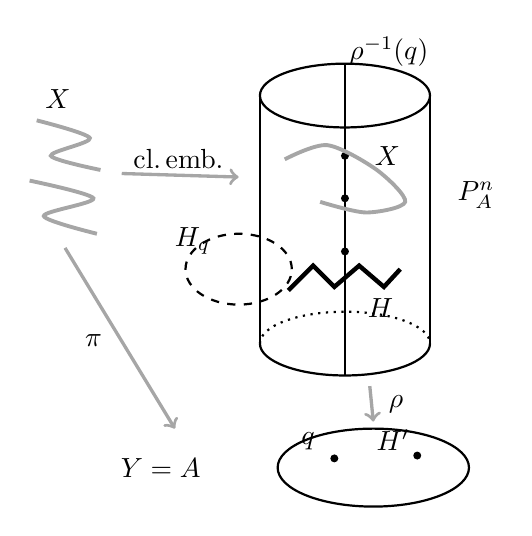
\begin{tikzpicture}[scale=0.9,line width=0.8pt]
  \draw (0,0.5) ellipse (1.2 and 0.45);
  \draw (-1.2,0.5) -- (-1.2,-3);
  \draw (1.2,0.5) -- (1.2,-3);
  \draw[dotted] (-1.2,-3) arc (180:0:1.2 and 0.45);
  \draw (-1.2,-3) arc (180:360:1.2 and 0.45);
  \node at (1.85,-0.9) {$\mathbb{P}^n_A$};
  \draw[thick] (0,0.95) -- (0,-3.45);
  \node at (0.62,1.12) {$\rho^{-1}(q)$};
  \fill (0,-0.35) circle (1.6pt);
  \fill (0,-0.95) circle (1.6pt);
  \fill (0,-1.7) circle (1.6pt);
  \draw[gray!70,line width=1.4pt] plot[smooth] coordinates {(-0.85,-0.4) (-0.25,-0.2) (0.45,-0.55) (0.85,-1.0) (0.3,-1.15) (-0.35,-1.0)};
  \node at (0.6,-0.35) {$X$};
  \draw[line width=1.6pt] (-0.8,-2.25) -- (-0.45,-1.9) -- (-0.15,-2.2) -- (0.2,-1.9) -- (0.55,-2.2) -- (0.78,-1.95);
  \node at (0.5,-2.5) {$H$};
  \draw[dashed] (-1.5,-1.95) ellipse (0.75 and 0.5);
  \node at (-2.15,-1.55) {$H_q$};
  \draw[gray!70,line width=1.4pt] plot[smooth] coordinates {(-4.35,0.15) (-3.6,-0.1) (-4.15,-0.35) (-3.45,-0.55)};
  \draw[gray!70,line width=1.4pt] plot[smooth] coordinates {(-4.45,-0.7) (-3.55,-0.95) (-4.25,-1.2) (-3.5,-1.45)};
  \node at (-4.05,0.45) {$X$};
  \draw[gray!70,line width=1.2pt,->] (-3.15,-0.6) -- (-1.5,-0.65);
  \node at (-2.35,-0.4) {$\mathrm{cl.\,emb.}$};
  \draw[gray!70,line width=1.2pt,->] (-3.95,-1.65) -- (-2.4,-4.2);
  \node at (-3.55,-2.95) {$\pi$};
  \draw (0.4,-4.75) ellipse (1.35 and 0.55);
  \fill (-0.15,-4.62) circle (1.6pt);
  \node at (-0.52,-4.38) {$q$};
  \fill (1.02,-4.58) circle (1.6pt);
  \node at (0.68,-4.36) {$H'$};
  \node at (-2.6,-4.75) {$Y=\Spec A$};
  \draw[gray!70,line width=1.2pt,->] (0.35,-3.6) -- (0.4,-4.1);
  \node at (0.72,-3.85) {$\rho$};
\end{tikzpicture}
\caption{\mbox{定理~18.1.6} 证明中的关键构造。（依原书手绘图重绘。）}\label{fig:finite-fibers-key-construction}
\end{figure}

\textbf{18.1.B.（练习：靶上纤维维数的\trUpperSemicontinuous{}性，就射影态射而言）}\quad 用与\mbox{定理~18.1.6} 中类似的手法，证明\emph{射影态射之纤维维数的\trUpperSemicontinuous{}性}（upper semicontinuity of fiber dimension of projective morphisms）：设 $\pi\colon X\to Y$ 是一个\trProjective\trMorphism，其中 $Y$ \trLocally\trNoetherian（或者更一般地，$\OO_Y$ 在自身上凝聚）。证明：$\{q\in Y\,:\,\dim\pi^{-1}(q)>k\}$ 是 $Y$ 的一个\trZariski\trClosedSubset。换言之，纤维的维数在靶的诸\trZariski\trClosedSubset{}上「跳跃」。（你可以把 $k=-1$ 的情形解读为「\trProjective\trMorphism{}都是闭的」这一事实——它基本上就是消元理论基本定理~8.4.10；参看 \S17.3.2。）这个练习对于体会\trProjective\trMorphism{}的行为方式而言相当重要。（\trVariety{}的情形早已在\mbox{定理~12.4.3(b)} 中做过；这条思路要简单得多。）

本节的最后一个练习则属另一个主题。

\textbf{18.1.C.（练习）}\quad 设 $0\to\mathscr{F}\to\mathscr{G}\to\mathscr{H}\to 0$ 是 $X$ 上诸\trQCSheaf{}的一个\trExactSequence，其中 $X$ 在 $A$ 上射影，而 $\mathscr{F}$ 凝聚。证明：当 $n\gg 0$ 时，
\[
0\longrightarrow \mathrm{H}^0(X,\mathscr{F}(n))\longrightarrow \mathrm{H}^0(X,\mathscr{G}(n))\longrightarrow \mathrm{H}^0(X,\mathscr{H}(n))\longrightarrow 0
\]
也正合。（提示：当 $n\gg 0$ 时，$\mathrm{H}^1(X,\mathscr{F}(n))=0$。）


\section{关键性质的定义与证明}

本节完全可以留待很久之后再读；我们将要用到的那些事实都已在上一节中陈述过了。不过，这些论证并不复杂，所以你不妨立刻就读。阅读时，你应当回过头去，把上一节中的那些事实逐条核对打钩，好让自己确信：所许诺的一切，你都懂得了。

\textbf{18.2.1. \trCechCohomology{}（Čech cohomology）。}\quad 一般框架下的\trCechCohomology{}是用对一空间越来越细的覆盖取极限来定义的。而在我们的代数几何框架中，情形要干净得多：我们可以只用单个覆盖。

设 $X$ \trQuasicompact{}且\trSeparated——例如当 $X$ 在 $A$ 上\trQuasiprojective{}时即如此。特别地，$X$ 可被有限多个\trAffine{}开集覆盖，且任意两个\trAffine{}开集之交仍是一个\trAffine{}开集（由\trSeparatedness，\mbox{命题~11.2.13}）。我们之所以使用\trQuasicompactness{}与\trSeparatedness，只是为了保证这两条好性质。

设 $\mathscr{F}$ 是一个\trQCSheaf，而 $\mathscr{U}=\{\mathfrak{U}_i\}_{i=1}^{n}$ 是由覆盖 $X$ 的\trAffine{}开集组成的一个\emph{有限}族。对 $I\subset\{1,\dots,n\}$，定义 $\mathfrak{U}_I=\bigcap_{i\in I}\mathfrak{U}_i$，由分离假设，它是\trAffine{}的。（对那些在其他背景下见过\trCohomology{}的读者，这里有一个极强的类比：用有限多个开集 $\mathfrak{U}_i$ 覆盖一个\trTopologicalSpace{} $X$，使得一切交 $\bigcap_{i\in I}\mathfrak{U}_i$ 都\trContractible。）考虑\textbf{\trCech\trComplexN}（Čech complex）
\begin{equation*}\tag{18.2.1.1}\label{eq:cech-complex}
\begin{aligned}
0\longrightarrow\prod_{\substack{|I|=1\\ I\subset\{1,\dots,n\}}}\mathscr{F}(\mathfrak{U}_I)\longrightarrow\cdots\longrightarrow{}\\
\prod_{\substack{|I|=i\\ I\subset\{1,\dots,n\}}}\mathscr{F}(\mathfrak{U}_I)\longrightarrow\prod_{\substack{|I|=i+1\\ I\subset\{1,\dots,n\}}}\mathscr{F}(\mathfrak{U}_I)\longrightarrow\cdots.
\end{aligned}
\end{equation*}

诸映射定义如下。除非 $I\subset J$（也就是说 $J=I\cup\{j\}$），否则从 $\mathscr{F}(\mathfrak{U}_I)\to\mathscr{F}(\mathfrak{U}_J)$ 的映射是 $0$。若 $j$ 是 $J$ 的第 $k$ 个元素，则该映射便是限制映射 $\mathrm{res}_{\mathfrak{U}_I,\mathfrak{U}_J}$ 的 $(-1)^{k-1}$ 倍。

\textbf{18.2.A.（容易的练习：致那些从未见过类似\trCech\trComplexN{}之物的读者）}\quad 证明：\trCech\trComplexN{}确实是一个\trComplexN，也就是说，相邻两支箭头的复合是 $0$。

定义 $\mathrm{H}^i_{\mathscr{U}}(X,\mathscr{F})$ 为复形 \eqref{eq:cech-complex} 的第 $i$ 个\trCohomology{}群。（指标从 $i=0$ 起算。）注意，若 $X$ 是一个 $A$-\trScheme，则 $\mathrm{H}^i_{\mathscr{U}}(X,\mathscr{F})$ 是一个 $A$-\trModule。我们差不多就要成功地定义出\trCechCohomology{}群 $\mathrm{H}^i$ 了，只可惜我们的定义先验地依赖于覆盖 $\mathscr{U}$ 的选取。注意，$\mathrm{H}^i_{\mathscr{U}}(X,\cdot)$ 显然是一个\trCovariantFunctor{} $\mathit{QCoh}_X\to\mathit{Mod}_A$。

\textbf{18.2.B.（容易的练习）}\quad 把 $\mathrm{H}^0_{\mathscr{U}}(X,\mathscr{F})$ 与 $\Gamma(X,\mathscr{F})$ 等同起来。（提示：使用 $\mathscr{F}$ 的\trSheaf{}公理。）

\textbf{18.2.C.（练习）}\quad 设
\begin{equation*}\tag{18.2.1.2}\label{eq:ses-sheaves-topological}
0\longrightarrow\mathscr{F}\longrightarrow\mathscr{G}\longrightarrow\mathscr{H}\longrightarrow 0
\end{equation*}
是一个\trTopologicalSpace{}上诸\trAbelianGroups{}层的\trShortExactSequence，而 $\mathscr{U}$ 是一个有限开覆盖，使得对 $\mathscr{U}$ 中诸开子集的任意交 $\mathfrak{U}_I$，映射 $\Gamma(\mathfrak{U}_I,\mathscr{G})\to\Gamma(\mathfrak{U}_I,\mathscr{H})$ 都是满射。证明：我们得到「$\mathrm{H}^i_{\mathscr{U}}$ 的\trCohomology{}\trLongExactSequence」（其中我们对 $\mathrm{H}^i_{\mathscr{U}}$ 采用同样的定义）。在我们的情形——$X$ 是一个\trQuasicompact\trSeparated{}的 $A$-\trScheme，而 \eqref{eq:ses-sheaves-topological} 是 $X$ 上诸\trQCSheaf{}的\trShortExactSequence——证明：我们得到 $A$-\trModule{} $\mathrm{H}^i_{\mathscr{U}}$ 的一个\trLongExactSequence。

在\mbox{定理~18.2.4}与\mbox{定理~18.7.1}的证明中，我们将用到你的连接同态构造所具有的一个特点：它将「与 $A$ 的局部化交换」。更精确地说，我们将需要下面这条练习。

\textbf{18.2.D.（练习）}\quad 设在\trQuasicompact\trSeparated{}的 $A$-\trScheme{} $\pi\colon X\to\Spec A$ 上给定诸\trQCSheaf{}的一个\trShortExactSequence{} \eqref{eq:ses-sheaves-topological}、由\trAffine{}开集组成的 $X$ 的一个覆盖 $\mathscr{U}$、以及某个 $f\in A$。把 $\mathscr{U}$ 的诸开集限制到 $X_f$ 上，便给出 $X_f=\pi^{-1}(\mathrm{D}(f))$ 的一个\trAffine{}开覆盖 $\mathscr{U}'$。请把「用 $\mathrm{H}^i_{\mathscr{U}}$ 并在 $f$ 处局部化而得到的、与 \eqref{eq:ses-sheaves-topological} 相伴的\trLongExactSequence」等同于「用\trAffine{}开覆盖 $\mathscr{U}'$ 而得到的、与 \eqref{eq:ses-sheaves-topological} 限制到 $X_f$ 上者相伴的\trLongExactSequence」。（先检验由协变性给出的那些映射——例如 $\mathrm{H}^i_{\mathscr{U}}(\mathscr{F})\to\mathrm{H}^i_{\mathscr{U}}(\mathscr{G})$——都「与局部化交换」，然后检验连接同态也如此。）

\textbf{18.2.2.\ \trhTheorem{}/\trhDefinition{。}}\ ——\ \emph{我们的\trStandingHypothesis{}是：$X$ \trQuasicompact{}且\trSeparated。$\mathrm{H}^i_{\mathscr{U}}(X,\mathscr{F})$ 不依赖于（有限）覆盖 $\{\mathfrak{U}_i\}$ 的选取。更精确地说，对任意两个覆盖 $\{\mathfrak{U}_i\}\subset\{V_i\}$，由\trCech\trComplexN{} \eqref{eq:cech-complex} 的自然映射所诱导的诸映射 $\mathrm{H}^i_{\{V_i\}}(X,\mathscr{F})\to\mathrm{H}^i_{\{\mathfrak{U}_i\}}(X,\mathscr{F})$ 都是\trIsomorphism。定义\textbf{\trCechCohomology{}群} $\mathrm{H}^i(X,\mathscr{F})$ 为这个群。}

如果你还不清楚「\trCech\trComplexN{}的自然映射」指的是什么，那么见到 \eqref{eq:les-complexes} 时它自会明朗。

\textbf{18.2.3.}\quad 致专家：在\trCohomology{}群上诱导出\trIsomorphism{}的那些复形间的映射称作\textbf{\trQuasiisomorphism}（quasiisomorphism）。由这个构造我们实际得到的，其实是比\trCohomology{}更细的不变量：我们得到的是 $A$-模的\emph{\trDerivedCategory}（derived category）中的一个元素。

\emph{证明。}\quad 只需在 $|\{V_i\}|=|\{\mathfrak{U}_i\}|+1$ 的情形证明该结果。我们将证明：若 $\{\mathfrak{U}_i\}_{1\le i\le n}$ 是 $X$ 的一个覆盖，而 $\mathfrak{U}_0$ 是任意另外一个\trAffine{}开集，则映射 $\mathrm{H}^i_{\{\mathfrak{U}_i\}_{0\le i\le n}}(X,\mathscr{F})\to\mathrm{H}^i_{\{\mathfrak{U}_i\}_{1\le i\le n}}(X,\mathscr{F})$ 是一个\trIsomorphism。考虑复形的如下\trExactSequence
\begin{equation*}\tag{18.2.3.1}\label{eq:les-complexes}
\begin{tikzcd}[row sep=2.9em, column sep=1.6em]
& 0 \ar[d] & 0 \ar[d] & 0 \ar[d] & \\
\cdots \ar[r] & \prod\limits_{\substack{|I|=i-1\\ 0\in I}}\mathscr{F}(\mathfrak{U}_I) \ar[r] \ar[d] & \prod\limits_{\substack{|I|=i\\ 0\in I}}\mathscr{F}(\mathfrak{U}_I) \ar[r] \ar[d] & \prod\limits_{\substack{|I|=i+1\\ 0\in I}}\mathscr{F}(\mathfrak{U}_I) \ar[r] \ar[d] & \cdots \\
\cdots \ar[r] & \prod\limits_{|I|=i-1}\mathscr{F}(\mathfrak{U}_I) \ar[r] \ar[d] & \prod\limits_{|I|=i}\mathscr{F}(\mathfrak{U}_I) \ar[r] \ar[d] & \prod\limits_{|I|=i+1}\mathscr{F}(\mathfrak{U}_I) \ar[r] \ar[d] & \cdots \\
\cdots \ar[r] & \prod\limits_{\substack{|I|=i-1\\ 0\notin I}}\mathscr{F}(\mathfrak{U}_I) \ar[r] \ar[d] & \prod\limits_{\substack{|I|=i\\ 0\notin I}}\mathscr{F}(\mathfrak{U}_I) \ar[r] \ar[d] & \prod\limits_{\substack{|I|=i+1\\ 0\notin I}}\mathscr{F}(\mathfrak{U}_I) \ar[r] \ar[d] & \cdots \\
& 0 & 0 & 0. &
\end{tikzcd}
\end{equation*}

通篇约定 $I\subset\{0,\dots,n\}$。下面两行是关于两个覆盖的\trCech\trComplexN，而二者之间的映射诱导出我们所想要的那个\trCohomology{}上的映射。从这个复形的\trShortExactSequence{}我们得到\trCohomology{}的\trLongExactSequence（\mbox{定理~1.5.8}）。于是我们希望证明顶行正合，从而其\trCohomology{}消失。（注意 $\mathfrak{U}_0\cap\mathfrak{U}_j$ 由我们的分离假设是\trAffine{}的，\mbox{命题~11.2.13}。）但顶行的第 $i$ 个\trCohomology{}恰恰是 $\mathrm{H}^{i-1}_{\{\mathfrak{U}_j\cap\mathfrak{U}_0\}_{j>0}}(\mathfrak{U}_0,\mathscr{F})$，唯独在起点处例外，那里我们得到 $0$（因为这个复形从 $0\to\mathscr{F}(\mathfrak{U}_0)\to\prod_{j=1}^{n}\mathscr{F}(\mathfrak{U}_0\cap\mathfrak{U}_j)$ 出发）。所以，只需证明仿射概形的更高次\trCech{}群是 $0$。于是由下述结果，证明即告完成。\hfill$\square$

\textbf{18.2.4.\ \trhTheorem{。}}\ ——\ \emph{\trAffine{} $A$-\trScheme{} $X$ 的更高次\trCechCohomology{} $\mathrm{H}^i_{\mathscr{U}}(X,\mathscr{F})$ 消失（对任意\trAffine{}覆盖 $\mathscr{U}$、$i>0$ 与\trQCSheaf{} $\mathscr{F}$）。}

这是又一次「\trPartitionOfUnity」式的论证，其精神与\mbox{定理~4.1.2}的证明如出一辙。

\emph{证明。}\quad 我们想证明「扩充」复形
\begin{equation*}\tag{18.2.4.1}\label{eq:extended-cech-complex}
0\longrightarrow\mathscr{F}(X)\longrightarrow\prod_{|I|=1}\mathscr{F}(\mathfrak{U}_I)\longrightarrow\prod_{|I|=2}\mathscr{F}(\mathfrak{U}_I)\longrightarrow\cdots
\end{equation*}
（即在开头添上了\trGlobalSections{} $\mathscr{F}(X)$）没有\trCohomology，也就是说，是正合的。（顺带一提，这个扩充复形称作 $\mathscr{F}(X)$ 的\textbf{\trCech{}分解}（Čech resolution），这里是相对于覆盖 $\mathscr{U}$ 的这一选取而言。）我们用一个技巧来做到这一点。

先设某个 $\mathfrak{U}_i$（比如说 $\mathfrak{U}_0$）就是 $X$。我们用障眼法来处理这种情形。\eqref{eq:extended-cech-complex} 这个复形正是下面这列复形的\trShortExactSequence{}的中间一行：
\begin{equation*}\tag{18.2.4.2}\label{eq:sleight-short-exact}
\begin{tikzcd}[row sep=3.4em, column sep=2em]
0 \ar[r] & 0 \ar[r] \ar[d] & \prod\limits_{|I|=1,0\in I}\mathscr{F}(\mathfrak{U}_I) \ar[r] \ar[d] & \prod\limits_{|I|=2,0\in I}\mathscr{F}(\mathfrak{U}_I) \ar[r] \ar[d] & \cdots \\
0 \ar[r] & \mathscr{F}(X) \ar[r] \ar[d] & \prod\limits_{|I|=1}\mathscr{F}(\mathfrak{U}_I) \ar[r] \ar[d] & \prod\limits_{|I|=2}\mathscr{F}(\mathfrak{U}_I) \ar[r] \ar[d] & \cdots \\
0 \ar[r] & \mathscr{F}(X) \ar[r] & \prod\limits_{|I|=1,0\notin I}\mathscr{F}(\mathfrak{U}_I) \ar[r] & \prod\limits_{|I|=2,0\notin I}\mathscr{F}(\mathfrak{U}_I) \ar[r] & \cdots
\end{tikzcd}
\end{equation*}
顶行就是底行向左平移一格的结果。相应的\trCohomology{}\trLongExactSequence{}表明，中间一行的\trCohomology{}消失。（你应当自行证明\trCohomology{}上的「连接同态」确实是一个\trIsomorphism。）这或许会让你想起\trMappingCone{}构造（\mbox{练习~1.6.E}）。（这里还有一个技巧，能从另一个角度达成这一段的目标。设 $\mathrm{id}$ 是复形 \eqref{eq:extended-cech-complex} 与其自身之间的恒等映射，又设 $0$ 是复形 \eqref{eq:extended-cech-complex} 与其自身之间的零映射。请描述 $\mathrm{id}$ 与 $0$ 之间的一个显式\trHomotopy；参 \S1.5.7。这个\trHomotopy{}将用到与 \eqref{eq:les-complexes} 相同的「想法」。于是，\trHomology{}上的恒等映射便等于\trHomology{}上的零映射（\mbox{练习~1.5.E}），故\trHomology{}必为零。这个想法颇有启发性，因为它还会在其他场合被用到。）

\begin{figure}[htbp]
\centering
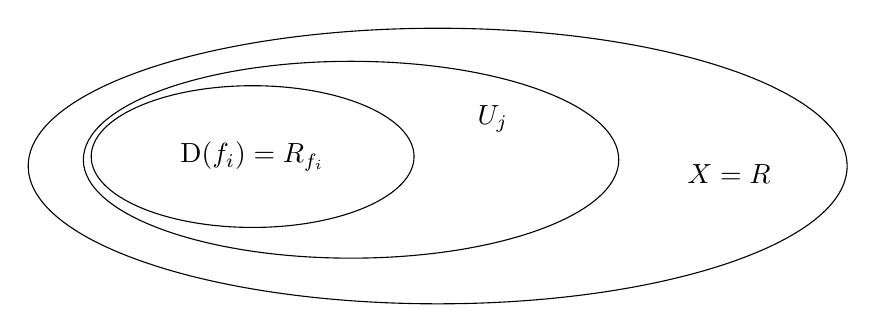
\begin{tikzpicture}[line join=round]
\draw (0,0) ellipse (5.2 and 1.75);
\draw (-1.1,0.08) ellipse (3.4 and 1.25);
\draw (-2.35,0.12) ellipse (2.05 and 0.9);
\node at (-2.35,0.12) {$\mathrm{D}(f_i)=\Spec R_{f_i}$};
\node at (0.7,0.6) {$\mathfrak{U}_j$};
\node at (3.7,-0.1) {$X=\Spec R$};
\end{tikzpicture}
\caption{\mbox{定理~18.2.2} 证明的最后一步。（依原书手绘图重绘。）}\label{fig:cech-final-step}
\end{figure}

最后，我们用再一记障眼法证明一般情形。设 $X=\Spec R$。我们想证明 $A$-模复形 \eqref{eq:extended-cech-complex} 是正合的。它同时也是 $R$-模的复形，于是我们想证明 $R$-模复形 \eqref{eq:extended-cech-complex} 是正合的。为证其正合，只需证明：对 $\Spec R$ 的由特异开集 $\mathrm{D}(f_i)$（$1\le i\le r$）组成的一个覆盖（也就是说 $(f_1,\dots,f_r)=1$ 于 $R$ 中），该复形是正合的。（翻译一下：层的序列的正合性可以局部检验。）我们如此选取覆盖，使得每个 $\mathrm{D}(f_i)$ 都含于我们的某个\trAffine{}开子集 $\mathfrak{U}_j$ 之中（见图~\ref{fig:cech-final-step}）。把复形 \eqref{eq:extended-cech-complex} 在 $f_i$ 处局部化，便得到 $\mathrm{D}(f_i)$ 关于其\trAffine{}覆盖 $\{\mathfrak{U}_k\cap\mathrm{D}(f_i)\}$ 的\trCech\trComplexN。我们要证明这个复形（对固定的 $i$ 与 $j$）是正合的。但这正是上一段处理过的情形——诸\trAffine{}开集之一，$\mathfrak{U}_j\cap\mathrm{D}(f_i)$，就等于 $\mathrm{D}(f_i)$。\hfill$\square$

至此，我们已证明了前一节的性质 \textbf{(i)--(iii)}。「仿射覆盖上同调消失」这条性质 \textbf{(vi)} 也同样直截了当：若 $X$ 被 $n$ 个\trAffine{}开集覆盖，就拿这些开集来充当覆盖 $\mathscr{U}$，并注意到\trCech\trComplexN{}在第 $n$ 步就终结了。

\textbf{18.2.E.（练习：性质 (v)）}\quad 设 $\pi\colon X\to Y$ 是一个\trAffine\trMorphism，$Y$ 是一个\trQuasicompact{}且\trSeparated{}的 $A$-\trScheme（从而 $X$ 亦是如此，因为\trAffine{}\trMorphism{}既\trQuasicompact{}又\trSeparated）。若 $\mathscr{F}$ 是 $X$ 上的一个\trQCSheaf，请描述一个自然的\trIsomorphism
$\mathrm{H}^i(Y,\pi_*\mathscr{F})\overset{\sim}{\longleftarrow}\mathrm{H}^i(X,\mathscr{F})$。（提示：若 $\mathscr{U}$ 是 $Y$ 的一个\trAffine{}覆盖，则「$\pi^{-1}(\mathscr{U})$」就是 $X$ 的一个\trAffine{}覆盖。用这两个覆盖来计算 $\mathscr{F}$ 的\trCohomology。）

\textbf{18.2.F.（练习：性质 (iv)）}\quad 设 $\pi\colon X\to Y$ 是任意一个\trQuasicompact\trSeparated{}\trMorphism，$\mathscr{F}$ 是 $X$ 上的一个\trQCSheaf，而 $Y$ 是一个\trQuasicompact\trSeparated{}的 $A$-\trScheme。对 $\pi$ 的这些假设保证 $\pi_*\mathscr{F}$ 是 $Y$ 上的一个\trQCSheaf。请描述一个自然的态射 $\mathrm{H}^i(Y,\pi_*\mathscr{F})\to\mathrm{H}^i(X,\mathscr{F})$，它是 $\Gamma(Y,\pi_*\mathscr{F})\to\Gamma(X,\mathscr{F})$ 的扩充。（旁注：这个态射在 $i=0$ 时是\trIsomorphism，但在更高的 $i$ 处未必是：考虑 $i=1$、$X=\mathbb{P}^1_k$、$\mathscr{F}=\OO(-2)$，而取 $Y$ 为一点 $\Spec k$。）

\textbf{18.2.G.（练习）}\quad 证明前一节的性质 \textbf{(vii)}，即「\trCohomology{}与\trFiltered\trColimit{}交换」。（这件事可以徒手完成。提示：在环上模的范畴中，对一个滤过集们取余极限是一个正合函子，\S1.5.14。）\footnote{原书此处作「taking the colimit over a filtered sets」，语法不通，疑当为「over a filtered set」之误，兹照录原书。——译者注}

至此，前一节的性质我们已尽数证毕，唯有 \textbf{(viii)} 除外，它将在 \S18.3 中处理。

\textbf{18.2.5. $k$-\trScheme{}上关于\trCohomology{}的若干有用事实。}

\textbf{18.2.H.（练习：\trCohomology{}与基域的变换）}\quad 设 $X$ 是一个\trQuasicompact\trSeparated{}的 $k$-\trScheme，$\mathscr{F}$ 是 $X$ 上的一个\trQCSheaf。给出一个对一切 $i$ 成立的\trIsomorphism
\[
\mathrm{H}^i(X,\mathscr{F})\otimes_k K\overset{\sim}{\longleftarrow}\mathrm{H}^i(X\times_{\Spec k}\Spec K,\mathscr{F}\otimes_k K)
\]
其中 $K/k$ 是任意一个\trFieldExtension。这里 $\mathscr{F}\otimes_k K$ 指的是 $\mathscr{F}$ 拉回到 $X\times_{\Spec k}\Spec K$ 上的结果。于是 $h^i(X,\mathscr{F})=h^i(X\times_{\Spec k}\Spec K,\mathscr{F}\otimes_k K)$。（这条同构对「把关于 $k$-\trScheme{}的事实过渡为关于代数闭域上概形的事实」很有用。你的证明或许会以一种根本的方式用到\trVectorSpace{}——也就是说，线性代数。若果真没用到，那么，当 $k\to K$ 被换成一个平坦\trRingMorphism{} $B\to A$ 时，你仍可以证明一个更一般的结论。回忆一下：$B\to A$ 称作平坦的，若 $\otimes_B A$ 是一个正合函子 $\mathit{Mod}_B\to\mathit{Mod}_A$。给这条更难的练习一个提示：\mbox{FHHF 定理}，\mbox{练习~1.5.I}。至于下一步的推广，见\mbox{练习~18.7.B(b)}。）

\textbf{18.2.I.（练习：无基点性与基域扩张无关）}\quad 设 $X$ 是一个\trQuasicompact\trSeparated{}的 $k$-\trScheme，$\mathscr{L}$ 是 $X$ 上的一个\trInvertibleSheaf，而 $K/k$ 是一个\trFieldExtension。证明：$\mathscr{L}$ 是\trBasePointFree{}的，当且仅当它拉回到 $X\times_{\Spec k}\Spec K$ 上是\trBasePointFree{}的。（提示：取 $i=0$ 的\mbox{练习~18.2.H}表明：$\mathscr{L}$ 在 $k$ 上的诸\trSection{}的一个基，在与 $K$ 作张量之后，便成为 $\mathscr{L}\otimes_k K$ 的诸\trSection{}的一个基。）

\textbf{18.2.6.\ \trhTheorem{}（射影 $k$-\trScheme{}上诸\trQCSheaf{}的维数\trCohomology{}消失）。}\ ——\ \emph{设 $X$ 是一个\trProjective{} $k$-\trScheme，$\mathscr{F}$ 是 $X$ 上的一个\trQCSheaf。则当 $i>\dim X$ 时，$\mathrm{H}^i(X,\mathscr{F})=0$。}

换言之，\trCohomology{}在高于 $X$ 之\trDimension{}的一切次数上都消失。

\emph{证明。}\quad 设 $X\hookrightarrow\mathbb{P}^N$，并令 $n=\dim X$。我们来证明 $X$ 可以被 $n+1$ 个\trAffine{}开集覆盖。\mbox{练习~12.3.D} 表明：$\mathbb{P}^N$ 上存在 $n+1$ 个\trEffectiveCartierDivisor，使得它们的\trComplement{} $\mathfrak{U}_0,\dots,\mathfrak{U}_n$ 覆盖 $X$。于是 $\mathfrak{U}_i$ 是\trAffine{}的，从而 $\mathfrak{U}_i\cap X$ 是\trAffine{}的，这样我们便用 $n+1$ 个\trAffine{}开集覆盖了 $X$。\hfill$\square$

（事实证明，$n+1$ 个\trAffine{}开集总是必需的。证明这一点的途径之一，是证明稠密\trAffine{}开子集的\trComplement{}总是纯余维数 $1$ 的；例如见 [RotV, Lem.~2.3]。）

\textbf{18.2.7.}\ \hard\ \textbf{更一般情形的维数\trCohomology{}消失。}\quad 借助\trBlowup{}的理论，\mbox{定理~18.2.6} 可以被推广到拟射影 $k$-\trScheme；见 \S22.4.15。维数\trCohomology{}消失甚至在一般得多的框架下也成立。为了陈述它，我们需要用\trDerivedFunctor{}（第 23 章）这套更一般的机器来定义\trCohomology。若 $X$ 是一个\trNoetherian\trTopologicalSpace（\S3.6.14），而 $\mathscr{F}$ 是 $X$ 上任意一个阿贝尔群的层，则对一切 $i>\dim X$ 都有 $\mathrm{H}^i(X,\mathscr{F})=0$。（\trGrothendieck{}在 [GrS, pp.~29--30] 中勾勒了他那优雅的证明；更详细的讲解见 [Ha1, Theorem~III.2.7]。）特别地，若 $X$ 是一个\trDimension{}为 $n$ 的 $k$-\trVariety，则我们\emph{总是}有维数\trCohomology{}消失，甚至对那些疯狂到无法用 $n+1$ 个\trAffine{}开子集覆盖的簇也是如此（见 \S22.4.15）。


\section{射影空间上线丛的上同调}

我们终于要来证明关于\trCohomology{}的最后一条许诺过的基本事实，即 \S18.1 中的性质 \textbf{(viii)}（\mbox{定理~18.1.2}）：射影空间上线丛的\trCohomology。但在此之前，我们先讨论一个看似不同的问题：去掉原点的\trAffine{}空间之\trStructureSheaf{}的\trCohomology。

\textbf{18.3.1.}\ \emph{问题。}\quad 对任意环 $A$，设 $X=\mathbb{A}^{n+1}_A\setminus V(x_0,\dots,x_n)$，其中 $n\ge 1$。这里 $\mathbb{A}^{n+1}$ 上的坐标便是 $x_0,\dots,x_n$，如此下标的用意很快就会明白。试求 $\mathrm{H}^i(X,\OO_X)$。

\textbf{18.3.2.}\ \emph{答案。}\quad 我们将证明：除非 $i=0$（此时它将是 $A[x_0,\dots,x_n]$）或 $i=n$，否则 $\mathrm{H}^i(X,\OO_X)=0$。我们将会看到，$\mathrm{H}^n(X,\OO_X)$ 可以与形如下式的那些「Laurent 多项式」（Laurent polynomials）相等同：$(x_0x_1\cdots x_n)^{-1}A[x_0^{-1},x_1^{-1},\dots,x_n^{-1}]$。（这给出了「$\mathbb{A}^2_k\setminus\{(0,0)\}$ 不是\trAffine{}的」的又一个证明；参看 \S4.4.3。）（另请参看\trSerre{}的仿射性\trCohomology{}判别法，\S18.8.4。）

$X$ 有一个自然的\trOpenCover{} $\{\mathfrak{U}_i\}$，其中 $\mathfrak{U}_i=\mathrm{D}(x_i)$，我们就使用与之相应的\trCech\trComplexN。

我们讨论 $n=2$ 的情形，因为一切复杂之处都在这里现身。此时\trCech\trComplexN{}为
\begin{equation*}\tag{18.3.2.1}\label{eq:cech-complex-n2}
\begin{aligned}
0\longrightarrow A[x_0,x_1,x_2,x_0^{-1}]\times A[x_0,x_1,x_2,x_1^{-1}]\times A[x_0,x_1,x_2,x_2^{-1}]\longrightarrow{}\\
A[x_0,x_1,x_2,x_0^{-1},x_1^{-1}]\times A[x_0,x_1,x_2,x_1^{-1},x_2^{-1}]\times A[x_0,x_1,x_2,x_0^{-1},x_2^{-1}]\longrightarrow{}\\
A[x_0,x_1,x_2,x_0^{-1},x_1^{-1},x_2^{-1}]\longrightarrow 0.
\end{aligned}
\end{equation*}

我们如此扩充 \eqref{eq:cech-complex-n2}：把左端的「$0\to$」换成「$0\to A[x_0,x_1,x_2]\to$」：
\begin{equation*}\tag{18.3.2.2}\label{eq:extended-complex-n2}
\begin{tikzcd}[row sep=2.6em, column sep=1.55em]
& \mathrm{H}^0 & \mathfrak{U}_0\ \mathfrak{U}_1\ \mathfrak{U}_2 & & \mathfrak{U}_{012} & \\
0 \ar[r] & A[x_0,x_1,x_2] \ar[r] & \cdots \ar[r] & \cdots \ar[r] & A[x_0,x_1,x_2,x_0^{-1},x_1^{-1},x_2^{-1}] \ar[r] & 0.
\end{tikzcd}
\end{equation*}

\textbf{18.3.A.（练习）}\quad 证明：若 \eqref{eq:extended-complex-n2} 正合，唯独在 $\mathfrak{U}_{012}$ 处的\trCohomology{}/余核是 $x_0^{-1}x_1^{-1}x_2^{-1}A[x_0^{-1},x_1^{-1},x_2^{-1}]$，则\mbox{答案~18.3.2} 对 $n=2$ 是正确的。

由于 \eqref{eq:extended-complex-n2} 中的诸映射保持多重次数（multidegree）——也就是说，每个 $x_i$ 的次数各自独立地保持——我们可以按\trMonomial{}逐一研究 \eqref{eq:extended-complex-n2} 的正合性。

\emph{「3 个负指数」的情形。}\quad 先考虑\trMonomial{} $x_0^{a_0}x_1^{a_1}x_2^{a_2}$，其中诸指数 $a_i$ 全为负数。此时 \eqref{eq:extended-complex-n2} 在这个多重次数下为：
\[
0\longrightarrow 0_{\mathrm{H}^0}\longrightarrow 0_0\times 0_1\times 0_2\longrightarrow 0_{01}\times 0_{12}\times 0_{02}\longrightarrow A_{012}\longrightarrow 0.
\]
这里的下标只是提醒我们，各个因子对应于哪个「\trCech{}」项。例如，$A_{012}$ 对应的是 $x_0^{a_0}x_1^{a_1}x_2^{a_2}$ 在 $A[x_0,x_1,x_2,x_0^{-1},x_1^{-1},x_2^{-1}]$ 中的系数。显然，这个复形只在 $\mathfrak{U}_{012}$ 那一处有（上）\trHomology，正如所愿。

\emph{「2 个负指数」的情形。}\quad 接下来考虑两个指数（比如说 $a_0$ 与 $a_1$）为负数的情形。此时该复形在这个多重次数下为
\[
0\longrightarrow 0_{\mathrm{H}^0}\longrightarrow 0_0\times 0_1\times 0_2\longrightarrow A_{01}\times 0_{12}\times 0_{02}\longrightarrow A_{012}\longrightarrow 0,
\]
显然正合。

\emph{「1 个负指数」的情形。}\quad 我们接下来考虑其中一个指数（比如说 $a_0$）为负数的情形。此时该复形在这个多重次数下为
\[
0\longrightarrow 0_{\mathrm{H}^0}\longrightarrow A_0\times 0_1\times 0_2\longrightarrow A_{01}\times 0_{12}\times A_{02}\longrightarrow A_{012}\longrightarrow 0.
\]
稍加思考（留意那些箭头 $A\to A$ 上的符号），你就会看出它是正合的。（这些下标提醒我们原\trCech\trComplexN{}中的下标，从而提醒我们在诸映射中该取什么符号。）

\emph{「0 个负指数」的情形。}\quad 最后，考虑诸指数皆不为负的情形。此时该复形在这个多重次数下为
\begin{equation*}\tag{18.3.2.3}\label{eq:multidegree-zero-negative}
0\longrightarrow A_{\mathrm{H}^0}\longrightarrow A_0\times A_1\times A_2\longrightarrow A_{01}\times A_{12}\times A_{02}\longrightarrow A_{012}\longrightarrow 0.
\end{equation*}

我们想证明它是正合的。我们采用在 \eqref{eq:sleight-short-exact} 处用过的同一策略：把 \eqref{eq:multidegree-zero-negative} 写成诸复形的一个\trShortExactSequence{}的中间一行：
\begin{equation*}\tag{18.3.2.4}\label{eq:ses-complexes-multidegree}
\begin{tikzcd}[row sep=3.0em, column sep=1.5em]
0 \ar[r] \ar[d] & 0 \ar[r] \ar[d] & A_2 \ar[r] \ar[d] & A_{02}\times A_{12} \ar[r] \ar[d] & A_{012} \ar[r] \ar[d] & 0 \ar[d] \\
0 \ar[r] \ar[d] & A_{\mathrm{H}^0} \ar[r] \ar[d] & A_0\times A_1\times A_2 \ar[r] \ar[d] & A_{01}\times A_{12}\times A_{02} \ar[r] \ar[d] & A_{012} \ar[r] \ar[d] & 0 \ar[d] \\
0 \ar[r] & A_{\mathrm{H}^0} \ar[r] & A_0\times A_1 \ar[r] & A_{01} \ar[r] & 0 \ar[r] & 0.
\end{tikzcd}
\end{equation*}

于是我们得到\trCohomology{}的\trLongExactSequence（\mbox{定理~1.5.8}）。但顶行与底行都是正合的（基本上来自「1 个负指数」的情形），也就是说不含\trCohomology，故中间一行也必定正合。（另一种做法：如 \eqref{eq:sleight-short-exact} 那样，设 $\mathrm{id}$ 是复形 \eqref{eq:multidegree-zero-negative} 与其自身之间的恒等映射。请描述 $\mathrm{id}$ 与零映射之间的一个显式\trHomotopy。那么\trHomology{}上的恒等映射便等于\trHomology{}上的零映射（\mbox{练习~1.5.E}），这就意味着\trHomology{}为零。）

\textbf{18.3.B.（练习）}\quad 证明：\mbox{答案~18.3.2} 对一切 $n\ge 1$ 都成立。（我当然本可以直接给出一般 $n$ 的证明，但亲眼看到这套论证运转起来或许更有启发。特别是，你的论证可能要短得多。例如，「2 个负指数」的情形可以照「1 个负指数」的情形那样处理，所以只要你安排得当，其实并不需要 $n+1$ 个分开的情形。）

\textbf{18.3.3.}\ \emph{\trhRemark{}。}\quad 这套论证基本上就是下述结论的证明：单形（simplex）$S$ 的\trBoundary{}（在某些圈子里被称作『球面』）的约化同调（reduced homology）是 $0$，除非 $S$ 是空集——在那种情形，它是一维的。\footnote{译注：原文 circles 一语双关：既指「圈子」，也暗合「圆」，与「球面」相映成趣。}「空集」的情形对应于「3 个负指数」的情形。

现在我们已准备好证明\mbox{定理~18.1.2}了。

\textbf{18.3.4.}\ \emph{\mbox{定理~18.1.2} 的证明。}\quad 我们使用 $\mathbb{P}^n_A$ 的标准覆盖 $\mathfrak{U}_0=\mathrm{D}(x_0)$，…，$\mathfrak{U}_n=\mathrm{D}(x_n)$。

我们来到了那个核心技巧（\mbox{练习~18.3.C}）：$\OO(m)$ 的\trCech\trComplexN{}就是 $\mathrm{H}^i(\mathbb{A}^{n+1}_A,\OO_X)$ 的\trCech\trComplexN{}的次数 $m$ 部分！（如果有帮助的话，你可以盯着 $n=2$ 的情形 \eqref{eq:cech-complex-n2} 看。）

\textbf{18.3.C.（练习；参看\mbox{注记~18.3.5}）}\quad 设 $I\subset\{0,\dots,n\}$，请给出 $\Gamma(\mathfrak{U}_I,\OO(m))$ 与那些 $m$ 次\trHomogeneous{}的 Laurent 单项式（于 $x_0,\dots,x_n$ 中，以 $A$ 为系数，其中每个满足 $i\notin I$ 的 $x_i$ 都以非负次数出现）之间的一个同构（作为 $A$-\trModule{}的同构）。你的构造应当使得限制映射 $\Gamma(\mathfrak{U}_I,\OO(m))\to\Gamma(\mathfrak{U}_J,\OO(m))$（$I\subset J$）对应于自然的包含关系：$\Gamma(\mathfrak{U}_I,\OO(m))$ 中的一个 Laurent 多项式被映到 $\Gamma(\mathfrak{U}_J,\OO(m))$ 中\emph{同一个} Laurent 多项式。

\textbf{18.3.D.（练习）}\quad 证明\mbox{定理~18.1.2}。\hfill$\square$

\textbf{18.3.5.}\ \emph{\trhRemark{}。}\quad \mbox{练习~15.1.C} 与 \mbox{练习~15.1.D} 曾把 $\mathrm{H}^0(\mathbb{P}^n_A,\OO_{\mathbb{P}^n_A}(m))$ 解释为 $x_0,\dots,x_n$ 中 $m$ 次\trHomogeneous{}的多项式（以 $A$ 为系数）。现在我们可以用更好的方式来陈述这件事。设
\[
\pi\colon\mathbb{A}^{n+1}_A\setminus V(x_0,\dots,x_n)\longrightarrow\mathbb{P}^n_A
\]
是\mbox{练习~7.3.F} 与\mbox{例~7.3.12} 的那个\trMorphism。你可以证明，诱导映射
\[
\pi^*\colon\mathrm{H}^n(\mathbb{P}^n_A,\OO(m))\longrightarrow\mathrm{H}^n(\mathbb{A}^{n+1}_A\setminus V(x_0,\dots,x_n),\OO)
\]
是一个\trInclusionMap，并请「辨识出它的像」。


\section{\trRiemannRoch{}与\trArithmeticGenus}

我们已经见识过\trCechCohomology{}的一些强大用法：证明关于\trGlobalSections{}空间的事情，以及证明\trSerre{}消失。现在我们将会看到，一些经典的构造可以来得又快又便宜。

本节中，我们在一个域 $k$ 上工作。设 $\mathscr{F}$ 是\trProjective{} $k$-\trScheme{} $X$ 上的一个\trCoherentSheaf。回忆记号（\S18.1）$h^i(X,\mathscr{F}):=\dim_k\mathrm{H}^i(X,\mathscr{F})$。由\mbox{定理~18.1.3}，$h^i(X,\mathscr{F})$ 是有限的。（一旦我们经由\trGrothendieck{}凝聚定理~\mbox{18.9.1} 对固有态射得到了这种有限性，本节的论证便可不加改变地推广到\trProper{}的 $X$ 上。）定义 $\mathscr{F}$ 的\textbf{\trEulerCharacteristic}（Euler characteristic）为
\[
\chi(X,\mathscr{F}):=\sum_{i=0}^{\dim X}(-1)^i h^i(X,\mathscr{F}).
\]
在这里与往后我们会反复看到：\trEulerCharacteristic{}比个别的\trCohomology{}群表现得更规矩。一个迹象是：注意，对固定的 $n$ 与 $m\ge 0$，
\[
h^0(\mathbb{P}^n_k,\OO(m))=\binom{n+m}{m}=\frac{(m+1)(m+2)\cdots(m+n)}{n!}.
\]
注意，右边的表达式是变元 $m$ 的一个 $n$ 次多项式。（为备日后参考，也请注意其首项是 $m^n/n!$。）但是，
\[
h^0(\mathbb{P}^n_k,\OO(m))=\frac{(m+1)(m+2)\cdots(m+n)}{n!}
\]
并非对\emph{一切} $m$ 都成立——当 $m\le -n-1$ 时失效。不过你仍可以验证（用\mbox{定理~18.1.2}）：
\[
\chi(\mathbb{P}^n_k,\OO(m))=\frac{(m+1)(m+2)\cdots(m+n)}{n!}.
\]
所以便有这一课：若某个\trCohomology{}群（通常是最高的或最低的那个）在某段范围内表现良好，随后却乱了套，那么多半是因为（i）其实\emph{始终}表现良好的乃是\trEulerCharacteristic，以及（ii）其余的\trCohomology{}群在那段范围内全都消失。

事实上我们将会看到：计算\trCohomology{}群（连 $h^0$ 在内）往往很难，而计算\trEulerCharacteristic{}却可能容易些。因此，把握\trCohomology{}群的一条重要途径便是：先算出\trEulerCharacteristic，再证明\emph{其余}的\trCohomology{}群全都消失。\emph{消失定理}（vanishing theorems）之所以无处不在又举足轻重，道理即在于此。（一条消失定理通常是说：某个\trCohomology{}群在某些条件下消失。）在讨论曲线时，我们就会看到它在起作用。（最早的应用之一将是 \mbox{(19.2.5.1)}。）

下面的练习表明\trEulerCharacteristic{}表现良好的另一种方式：\emph{它在\trExactSequence{}中是\trAdditive{}的}。

\textbf{18.4.A.（练习）}\quad 证明：若 $0\to\mathscr{F}\to\mathscr{G}\to\mathscr{H}\to 0$ 是\trProjective{} $k$-\trScheme{} $X$ 上诸\trCoherentSheaf{}的一个\trExactSequence，则 $\chi(X,\mathscr{G})=\chi(X,\mathscr{F})+\chi(X,\mathscr{H})$。（提示：考虑\trCohomology{}中的\trLongExactSequence。）更一般地，若
\[
0\longrightarrow\mathscr{F}_1\longrightarrow\cdots\longrightarrow\mathscr{F}_n\longrightarrow 0
\]
是诸\trCoherentSheaf{}的一个\trExactSequence，证明
\[
\sum_{i=1}^{n}(-1)^i\chi(X,\mathscr{F}_i)=0.
\]
（这条练习一方面推广了\mbox{练习~1.5.B} 的「正合」情形——考虑 $X=\Spec k$ 的情形——另一方面又在证明中用到它。）

\textbf{18.4.1. 射影曲线上\trLineBundle{}的\trRiemannRoch{}定理。}

\textbf{18.4.B.（重要练习：射影曲线上\trLineBundle{}的\trRiemannRoch{}定理（第一版））}\quad 设 $D=\sum_{p\in C^{\mathrm{reg}}}a_p[p]$ 是域 $k$ 上\trProjective{}（纯维数 $1$）\trCurve{} $C$ 上的一个\trDivisor（其中 $a_p\in\mathbb{Z}$，且除有限多个 $a_p$ 之外均为 $0$）。这里 $C^{\mathrm{reg}}$ 是 $C$ 的维数 $0$ 的\trRegular{}点。定义 $D$ 的\textbf{次数}为
\[
\deg D=\sum a_p\deg p.
\]
（点 $p$ 的次数定义于 \S5.3.8，即剩余域在 $k$ 上的\trFieldExtension{}的次数。）证明
\[
\chi(C,\OO_C(D))=\deg D+\chi(C,\OO_C)
\]
对 $\sum|a_p|$ 归纳（其中 $D=\sum a_p[p]$ 如上）。提示：为证 $\chi(C,\OO_C(D))=\deg p+\chi(C,\OO_C(D-p))$，用 $\OO_C(D)$ 去张量\trClosedSubscheme{}正合列~\mbox{(9.1.2.1)}
\[
0\longrightarrow\OO_C(-p)\longrightarrow\OO_C\longrightarrow\OO_{|p|}\longrightarrow 0
\]
并利用\trEulerCharacteristic{}在\trExactSequence{}中的加性（\mbox{练习~18.4.A}）。

由于\trRegular{}\trCurve{}上每个\trInvertibleSheaf{} $\mathscr{L}$ 都具有 $\OO_C(D)$（对某个 $D$）的形状（见 \S15.4），这条练习威力非常强大。

\textbf{18.4.2.}\ \emph{重要定义：射影曲线上\trLineBundle{}的次数（在 \S18.4.7 中推广）。}\quad 设 $\mathscr{L}$ 是 $k$ 上\trProjective{}\trCurve{} $C$ 上的一个\trInvertibleSheaf（我们对 $C$ 的\trRegularity，乃至\trReducedness，都不作任何假设！）。定义 $\mathscr{L}$ 的\textbf{次数}（记作 $\deg\mathscr{L}$ 或 $\deg_C\mathscr{L}$）为
\[
\deg\mathscr{L}:=\chi(C,\mathscr{L})-\chi(C,\OO_C).
\]
于是我们有了一个次数映射 $\deg\colon\mathrm{Pic}\,C\to\mathbb{Z}$。$C$ 上次数为 $d$ 的\trLineBundle{}全体记作 $\mathrm{Pic}^d\,C:=\deg^{-1}(d)$。

\textbf{18.4.C.（重要而容易的练习：除子的次数＝相应\trLineBundle{}的次数（证成\mbox{注记~16.3.8}））}\quad 设 $\mathscr{L}$ 是 $k$ 上\trProjective{}（纯维数 $1$）\trCurve{} $C$ 上的一个\trInvertibleSheaf，并设 $s$ 是 $\mathscr{L}$ 在 $C$ 上的一个非零\trRational{}\trSection，它在 $C$ 的一切\trSingularPoint{}处都是\trRegular{}的。令 $D$ 为 $s$ 的\trZeros{}与\trPole{}所成的\trDivisor：
\[
D:=\sum_{p\in C}v_p(s)[p].
\]
证明 $\deg\mathscr{L}=\deg D$。特别地，\trRegular{}\trCurve{}上\trLineBundle{}的次数可以这样计算：数一数\emph{任一}不在 $C$ 的某个分量上恒为零的有理截面的零点与极点。

接下来的几条练习给出一些有用的应用。

\textbf{18.4.D.（练习）}\quad 用上面的想法，为\mbox{练习~16.3.E}（射影曲线上的一个非零有理函数拥有同样个数的零点与极点，须以恰当的方式计数）给出一个新的解法。

\textbf{18.4.E.（练习）}\quad 设 $s_1$ 与 $s_2$ 是\trIrreducible\trRegular\trProjective{}\trCurve{} $C$ 上次数为 $d$ 的\trLineBundle{} $\mathscr{L}$ 的两个\trSection，它们没有公共零点。则 $s_1$ 与 $s_2$ 决定一个\trMorphism{} $\pi\colon C\to\mathbb{P}^1_k$。证明：$\pi$ 是\trFinite\trMorphism，且 $\pi$ 的次数为 $d$。（翻译一下：$C$ 上一个二维的、无基点的、次数 $d$ 的\trLinearSystem{}给出 $\mathbb{P}^1$ 的一个次数 $d$ 的\trFinite{}覆盖。）

\textbf{18.4.F.（练习：将在\mbox{练习~18.4.M} 中扩展）}\quad 若 $\mathscr{L}$ 与 $\mathscr{M}$ 是\trRegular\trProjective{}\trCurve{} $C$ 上的两个\trLineBundle，证明 $\deg(\mathscr{L}\otimes\mathscr{M})=\deg\mathscr{L}+\deg\mathscr{M}$。（提示：选取 $\mathscr{L}$ 与 $\mathscr{M}$ 的非零\trRational{}\trSection。）

\textbf{18.4.3.}\ \emph{注记：「次数」映射 $\mathrm{Pic}\to\mathbb{Z}$ 是同态。}\quad 于是，对（域 $k$ 上的）\trRegular\trProjective{}\trCurve{} $C$，次数映射 $\deg\colon\mathrm{Pic}\to\mathbb{Z}$ 是\trAbelianGroups{}的一个\trHomomorphism。（这一结果将在\mbox{练习~18.4.M} 中推广到 $k$ 上的一切\trProper{}\trCurve。）

\textbf{18.4.G.（练习）}\quad 设 $\pi\colon C\to C'$ 是\trIntegral\trProjective\trRegular{}\trCurve{}之间次数为 $d$ 的\trMorphism，而 $\mathscr{L}$ 是 $C'$ 上的一个\trInvertibleSheaf。证明：$\deg_C\pi^*\mathscr{L}=d\deg_{C'}\mathscr{L}$。提示：用 $\mathscr{L}$ 的任一非零\trRational{}\trSection{} $s$ 计算 $\deg_{C'}\mathscr{L}$，并用 $\pi^*\mathscr{L}$ 的\trRational{}\trSection{} $\pi^*s$ 计算 $\deg_C\pi^*\mathscr{L}$。注意：零点拉回为零点，极点拉回为极点。视你的进路而定，\mbox{练习~16.3.D} 或许帮得上忙。

\textbf{18.4.H.}\ \extrahard\ \textbf{（练习：次数的复解析解释；仅供分析背景足够者）}\quad 设 $X$ 是一条\trConnected\trRegular\trProjective{}复曲线。证明：次数映射是下列诸群同态的复合
\[
\begin{tikzcd}[column sep=2.6em]
\mathrm{Pic}\,X \ar[r] & \mathrm{Pic}\,X^{\mathrm{an}} \ar[r, "c_1"] & \mathrm{H}^2(X^{\mathrm{an}},\mathbb{Z}) \ar[r, "{\cap[X^{\mathrm{an}}]}"] & \mathrm{H}_0(X^{\mathrm{an}},\mathbb{Z}) \cong \mathbb{Z}.
\end{tikzcd}
\]
提示：对群 $\mathrm{Pic}\,X$ 的一个\trGenerator{} $\OO(p)$ 证明之，使用显式的\trTransitionFunction。（第一个映射曾在\mbox{练习~14.1.J} 中讨论过。第二个映射把一个\trLineBundle{}送到它的第一\trChern{}类（first Chern class），可以这样来解释：一个\trLineBundle{}的诸\trTransitionFunction{}给出 $\OO^*_{X^{\mathrm{an}}}$ 的一个\trCech{} $1$-\trCycle；这就给出一个映射 $\mathrm{Pic}\,X^{\mathrm{an}}\to\mathrm{H}^1(X^{\mathrm{an}},\OO^*_{X^{\mathrm{an}}})$。再把它与相应于\trExponentialSequence{}~\mbox{(2.4.9.1)} 的\trCohomology{}\trLongExactSequence{}中的映射 $\mathrm{H}^1(X^{\mathrm{an}},\OO^*_{X^{\mathrm{an}}})\to\mathrm{H}^2(X^{\mathrm{an}},\mathbb{Z})$ 组合起来，便得到第一\trChern{}类映射。）

\textbf{18.4.4. \trArithmeticGenus。}

受几何的推动（见下文的\mbox{奇迹~18.4.5}），我们定义维数 $n$ \trScheme{} $X$ 的\textbf{\trArithmeticGenus}（arithmetic genus）为 $p_a(X):=(-1)^n(\chi(X,\OO_X)-1)$。对\trAlgClosedField{}上的\trIntegral\trProjective{}\trCurve，$h^0(X,\OO_X)=1$（\S11.4.7），于是 $p_a(X)=h^1(X,\OO_X)$。（在更高维数，这是一个较不自然的观念。）

我们可以把曲线的\trRiemannRoch{}公式（\mbox{练习~18.4.B}）重述为：
\begin{equation*}\tag{18.4.4.1}\label{eq:riemann-roch-h0-h1}
h^0(C,\mathscr{L})-h^1(C,\mathscr{L})=\deg\mathscr{L}-p_a(C)+1.
\end{equation*}
这是\trRiemannRoch{}公式最常见的一种表述。

\textbf{18.4.5. 奇迹。}\quad 若 $C$ 是一条\trRegular\trIrreducible\trProjective{}复曲线，则相应的复解析对象——一个紧的\trRiemannSurface——有一种叫做\emph{\trGenus} $g$ 的概念，（不严格地说）它就是洞的个数（见图~\ref{fig:genus-3-riemann-surface}）。奇迹般地，在此情形 $g=p_a$（见\mbox{练习~21.4.I}）；因此之故，在讨论\trRegular{}（\trProjective\trIrreducible）曲线时，无论在什么域上，我们都常写 $g$ 来记 $p_a$。我们将在 \S18.6.7 中进一步讨论亏格，届时我们将能在许多有趣的情形计算它。（\trhWarning{}：$\mathbb{P}^1_\mathbb{C}$ 作为 $\mathbb{R}$-\trVariety{}的\trArithmeticGenus{}是 $-1$！）

\begin{figure}[htbp]
\centering
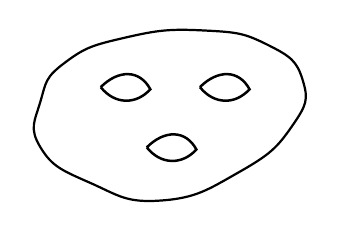
\begin{tikzpicture}[scale=0.9,line width=0.8pt]
  \draw[thick] plot[smooth cycle, tension=0.85] coordinates {
    (-1.7,0.55) (-1.35,1.1) (-0.5,1.45) (0.6,1.55) (1.5,1.35) (2.0,0.85) (1.85,0.2) (1.1,-0.45) (0.0,-0.85) (-1.0,-0.6) (-1.7,-0.1)};
  \draw[line width=0.9pt] (-0.85,0.75) .. controls (-0.6,1.0) and (-0.3,1.0) .. (-0.15,0.72) .. controls (-0.35,0.5) and (-0.65,0.5) .. (-0.85,0.75);
  \draw[line width=0.9pt] (0.55,0.75) .. controls (0.8,1.0) and (1.1,1.0) .. (1.25,0.72) .. controls (1.05,0.5) and (0.75,0.5) .. (0.55,0.75);
  \draw[line width=0.9pt] (-0.2,-0.1) .. controls (0.05,0.15) and (0.35,0.15) .. (0.5,-0.13) .. controls (0.3,-0.35) and (0.0,-0.35) .. (-0.2,-0.1);
\end{tikzpicture}
\caption{一个亏格 $3$ 的\trRiemannSurface{}。（依原书手绘图重绘。）}\label{fig:genus-3-riemann-surface}
\end{figure}

\textbf{18.4.6. \trCoherentSheaf{}的次数（例如\trVectorBundle{}的次数）。}

设 $C$ 是域 $k$ 上的一条\trIrreducible\trReduced{}\trCurve（可能奇异）。若 $\mathscr{F}$ 是 $C$ 上的一个\trCoherentSheaf，回忆一下（\S14.3.3）：$\mathscr{F}$ 的\emph{\trRank}（记作 $\operatorname{rank}\mathscr{F}$）是它在 $C$ 的\trGenericPoint{}处的\trRank。

\textbf{18.4.7.}\ \emph{\trhDefinition{。}}\quad 若 $C$ 是\emph{射影}的，定义 $\mathscr{F}$ 的\textbf{次数}为
\begin{equation*}\tag{18.4.7.1}\label{eq:degree-coherent-sheaf}
\deg\mathscr{F}=\chi(C,\mathscr{F})-(\operatorname{rank}\mathscr{F})\cdot\chi(C,\OO_C).
\end{equation*}
陈述 \eqref{eq:degree-coherent-sheaf} 常被称作射影曲线上\textbf{\trCoherentSheaf{}的\trRiemannRoch{}定理}（或\trVectorBundle{}的\trRiemannRoch{}定理）。

若 $\mathscr{F}$ 是一个\trInvertibleSheaf（或者，更一般地，若\trRank{}在每个\trIrreducibleComponent{}上都相同），我们便可以去掉\trIrreducibility{}假设。

\textbf{18.4.I.（容易的练习）}\quad 证明：次数（作为固定曲线 $C$ 上诸\trCoherentSheaf{}的函数）在\trExactSequence{}中是\trAdditive{}的。

\textbf{18.4.J.（练习）}\quad 若 $\mathscr{F}$ 是 $C$ 上的一个\trTorsion\trSheaf，证明 $\deg\mathscr{F}\ge 0$，且等号成立当且仅当 $\mathscr{F}=0$。

\textbf{18.4.K.（练习）}\quad 若 $k=\overline{k}$，而 $\mathscr{F}$ 是 $C$ 上的一个\trTorsion\trSheaf，证明 $\deg\mathscr{F}=\ell(\mathscr{F})$。（$\mathscr{F}$ 的\trLength{} $\ell(\mathscr{F})$ 定义于 \S6.5.8。）若 $k\ne\overline{k}$，会出什么岔子？

\textbf{18.4.L.}\ \hard\ \textbf{（练习）}\quad 设 $C$ 是域 $k$ 上的一个\trProjective{}\trCurve，$\mathscr{L}$ 是 $C$ 上的一个\trLineBundle，$\mathscr{F}$ 是 $C$ 上的一个\trCoherentSheaf。用下列步骤证明：$\chi(C,\mathscr{L}\otimes\mathscr{F})-\chi(C,\mathscr{F})$ 等于如下乘积对 $C$ 的各\trIrreducibleComponent{} $C_i$ 的求和：$\mathscr{L}$ 在 $C_i^{\mathrm{red}}$ 上的次数（\trReduction{}定义于 \S9.4.10）乘以 $\mathscr{F}$ 在 $C_i$ 的\trGenericPoint{} $\eta_i$ 处的\trLength（即 $\mathscr{F}_{\eta_i}$ 作为 $\OO_{\eta_i}$-\trModule{}的\trLength——\trLength{}定义于\mbox{定义~6.5.2}）。这条练习完全可以有理由称作\textbf{非既约曲线的\trRiemannRoch}。

（a）先化归到 $\mathscr{F}$ \trSchemeTheoretic{}支撑在 $C^{\mathrm{red}}$ 上的情形（有限型拟凝聚层的概形论支撑，你在\mbox{练习~9.1.N} 中定义过），做法是：证明所谓等式的两边在\trShortExactSequence{}中都是\trAdditive{}的，并使用 $\mathscr{F}$ 的如下\trFiltration
\[
0=\mathscr{I}^r\mathscr{F}\subset\mathscr{I}^{r-1}\mathscr{F}\subset\cdots\subset\mathscr{I}\mathscr{F}\subset\mathscr{F}
\]
（其中 $\mathscr{I}$ 是在 $C$ 中切出 $C^{\mathrm{red}}$ 的\trIdealSheaf）。于是我们只须考虑 $C$ 既约的情形。

（b）在这个「既约」情形中，由\mbox{练习~16.2.L}，我们可以写 $\mathscr{L}\cong\OO(\sum_j n_jp_j)$，其中诸 $p_j$ 是与 $\mathscr{F}$ 的\trAssociatedPoint{}互异的\trRegular{}点。用一道恰当的归纳法，证明剩下须证的部分。

\textbf{18.4.M.}\ \hard\ \textbf{（练习）}\quad 若 $\mathscr{L}$ 与 $\mathscr{M}$ 是域 $k$ 上\trProjective{}\trCurve{} $C$ 上的两个\trLineBundle，证明 $\deg_C(\mathscr{L}\otimes\mathscr{M})=\deg_C(\mathscr{L})+\deg_C(\mathscr{M})$。于是次数映射 $\deg\colon\mathrm{Pic}\,C\to\mathbb{Z}$ 是\trAbelianGroups{}的一个\trHomomorphism，这就把\mbox{注记~18.4.3} 加以推广。

\textbf{18.4.8.}\quad 事实上，$k$ 上一切\trProper{}\trCurve{}都是\trProjective{}的（\mbox{注记~19.2.I}），所以在\mbox{练习~18.4.L} 与~\mbox{练习~18.4.M} 中，「射影」可以换成「固有」。正是以这一面目，当我们讨论第 20 章的\trIntersectionTheory{}时，将会用到\mbox{练习~18.4.L}。

\textbf{18.4.9.}\ \emph{曲线上丰富丛的两条性质。}\quad 对于\mbox{练习~18.4.N} 与~\mbox{练习~18.4.O}，要么假设 $C$ 是\trRegular{}的（这样你就可以援引\mbox{注记~18.4.3}），要么使用带星的\mbox{练习~18.4.M}。

\textbf{18.4.N.（练习）}\quad 若 $C$ 是一个\trProjective{}\trCurve，而 $\mathscr{L}$ 是 $C$ 上的一个\trAmple\trLineBundle，证明 $\deg\mathscr{L}>0$。（提示：对 $\mathscr{L}$ \emph{\trVeryAmple}的情形证明之。）

\textbf{18.4.O.（练习）}\quad 设 $\mathscr{L}$ 是\trProper{}\trVariety{} $X$ 上的一个\trBasePointFree\trInvertibleSheaf，从而诱导出某个\trMorphism{} $\phi\colon X\to\mathbb{P}^n$。那么，$\mathscr{L}$ 是\trAmple{}的，当且仅当 $\phi$ 是\trFinite{}的。（提示：若 $\phi$ 是\trFinite{}的，用\mbox{练习~16.2.G}。若 $\phi$ 不是\trFinite{}的，用\mbox{定理~18.1.6} 证明存在一条被 $\phi$ 收缩的曲线 $C$。证明 $\mathscr{L}$ 在 $C$ 上的次数为 $0$。）

\textbf{18.4.10.}\ \hard\ \textbf{扩展例题：万有平面\trConic{}没有有理截面。}\quad 我们用次数的理论来得到一个有趣的推论。我们在一个取定的域 $k$ 上工作。考虑如下的图。
\begin{tikzcd}[row sep=2.8em, column sep=3.2em]
\mathscr{C} \ar[rd] \ar[r, "\mathrm{cl.\,emb.}"] & \mathbb{P}^2\times\mathbb{P}^5 \ar[d] \ar[r] & \mathbb{P}^2 \\
& \mathbb{P}^5 &
\end{tikzcd}
若 $\mathbb{P}^2$ 具有射影坐标 $x_0$、$x_1$、$x_2$，则 $\mathbb{P}^5$ 具有坐标 $a_{00}$、$a_{01}$、$a_{11}$、$a_{02}$、$a_{12}$、$a_{22}$，而 $\mathscr{C}$ 由单独一个方程
\[
a_{00}x_0^2+a_{01}x_0x_1+\cdots+a_{22}x_2^2=0
\]
切出。我们把 $\mathbb{P}^5$ 解释为（$\mathbb{P}^2$ 中的）\trConic{}的参数空间，把 $\mathscr{C}$ 解释为 $\mathbb{P}^5$ 之上的万有\trConic（它把一条\trConic{} $C$ 连同一点 $p\in C$ 一道参数化），并带有\trCanonical{}投射 $\mathscr{C}\to\mathbb{P}^2$。

\textbf{18.4.P.（练习）}\quad 把 $\mathscr{C}$ 解释为 $\mathbb{P}^2$ 上的 $\mathbb{P}^4$-丛（带有两个\trIrreducible\trDivisor，其\trComplement{}是 $\mathbb{A}^2$ 上的 $\mathbb{A}^4$-丛），证明：$\mathscr{C}$ 是一个光滑六维体，且 $\mathrm{Pic}\,\mathscr{C}\cong\mathbb{Z}\times\mathbb{Z}$。

\textbf{18.4.Q.（练习）}\quad 取定一条直线 $\ell\subset\mathbb{P}^2$ 与一个 $k$-值点 $q\in\mathbb{P}^2$。令 $D_\ell$ 为 $\mathscr{C}$ 上相应于 $(C,p)$（其中 $p$ 落在 $\ell$ 上）的\trDivisor。令 $D_q$ 为 $\mathscr{C}$ 上相应于 $(C,p)$（其中 $q\in C$）的\trDivisor。利用你对「$\mathscr{C}$ 是 $\mathbb{P}^2$ 上的 $\mathbb{P}^4$-丛」的描述，证明：$D_\ell$ 与 $D_q$ 生成 $\mathrm{Pic}\,\mathscr{C}$。

\textbf{18.4.R.（练习）}\quad 设 $K$ 是 $\mathscr{C}\to\mathbb{P}^5$ 在点 $r\in\mathbb{P}^5$ 之上的一根\trFiber——也就是说，域 $\kappa(r)$ 上 $\mathbb{P}^2$ 中的一条\trConic。再设 $K$ 是\trIntegral{}的，且 $q$ 与 $\ell$ 都不含于 $K$（这条假设并不必要，但可使问题简化）。证明：$\deg_K\OO(D_q)=0$ 且 $\deg_K\OO(D_\ell)=2$。进而证明：若 $\mathscr{L}$ 是 $\mathscr{C}$ 上的任一\trInvertibleSheaf，则 $\deg_K(\mathscr{L})$ 是偶数。

\textbf{18.4.S.（练习）}\quad 证明：投射 $\pi\colon\mathscr{C}\to\mathbb{P}^5$ 没有有理截面。提示：倘若在 $\mathbb{P}^5$ 的一个\trOpenSubset{} $\mathrm{U}$ 之上存在\trRegular{}\trSection，它将是 $\pi^{-1}(\mathrm{U})$ 上的一个\trDivisor；令 $D$ 为它在 $\mathscr{C}$ 中的\trClosure。证明：$D$ 与 $\pi$ 在 $\mathrm{U}$ 之上的任一\trFiber{}都以重数 $1$ 相交。用\mbox{练习~18.4.R} 导出矛盾。

我们可以按下面这种富于戏剧性的方式重述\mbox{练习~18.4.S}：没有办法写下三个关于 $a_{00},\dots,a_{22}$ 的有理函数 $X_0$、$X_1$、$X_2$，使得
\[
a_{00}X_0^2+a_{01}X_0X_1+\cdots+a_{22}X_2^2=0
\]
除非 $X_0=X_1=X_2=0$。

\trConic{}上有理点的存在问题是一个算术问题。（想想：$x^2+y^2=z^2$。）而我们的解法却是拓扑的。在这个例子中拓扑与算术的统一，是代数几何里一段漫长而富有成果的故事的开端。

\textbf{18.4.11.}\ \hard\ \textbf{\trNumericallyEquivalent、N\'eron--Severi 群、\trNef\trLineBundle、\trNef{}锥与丰富锥。}\quad 设 $X$ 是一个\trProper{} $k$-\trVariety，而 $\mathscr{L}$ 是 $X$ 上的一个\trInvertibleSheaf。若 $i\colon C\hookrightarrow X$ 是 $X$ 的一个一维\trClosed\trReduced{}\trSubscheme，则定义 $\mathscr{L}$ 在 $C$ 上的次数为 $\deg_C\mathscr{L}:=\deg_C i^*\mathscr{L}$。若对一切 $C$ 都有 $\deg_C\mathscr{L}=0$，我们便说 $\mathscr{L}$ 是\textbf{\trNumericallyTrivial}（numerically trivial）的。

\textbf{18.4.T.（练习）}\quad
（a）证明：$\mathscr{L}$ 是\trNumericallyTrivial{}的，当且仅当对 $X$ 中一切\emph{\trIntegral}曲线 $C$ 都有 $\deg_C\mathscr{L}=0$。

（b）证明：若 $\pi\colon X\to Y$ 是一个\trProper\trMorphism，而 $\mathscr{L}$ 是 $Y$ 上的一个\trNumericallyTrivial\trInvertibleSheaf，则 $\pi^*\mathscr{L}$ 在 $X$ 上\trNumericallyTrivial。

（c）证明：$\mathscr{L}$ 是\trNumericallyTrivial{}的，当且仅当 $\mathscr{L}$ 在 $X$ 的每个\trIrreducibleComponent{}上都\trNumericallyTrivial。

（d）证明：若 $\mathscr{L}$ 与 $\mathscr{L}'$ \trNumericallyTrivial，则 $\mathscr{L}\otimes\mathscr{L}'$ 与 $\mathscr{L}^\vee$ 都\trNumericallyTrivial。

\textbf{18.4.12.}\ \emph{\trNumericallyEquivalent。}\quad 由（d）部分，\trNumericallyTrivial\trInvertibleSheaf{}全体构成 $\mathrm{Pic}\,X$ 的一个子群，记作 $\mathrm{Pic}^\tau X$。模去\trNumericallyTrivial\trLineBundle{}所组成的子群而等价的两个线丛，称为\textbf{\trNumericallyEquivalent}（numerically equivalent）的。\footnote{原书此处作「Two lines bundles」，当为「Two line bundles」之误，径改。——译者注}在\trNumericallyEquivalent{}之下稳定的\trInvertibleSheaf{}性质，称为一个\emph{数值性质}（numerical property）。我们将会看到，「\trNef{}性」（nefness）与\trAmpleness{}都是数值性质（分别见\mbox{定义~18.4.13}与\mbox{注记~20.4.2}）。

日后将定义 $X$ 的\emph{N\'eron--Severi 群} $\mathrm{NS}(X)$ 为 $\mathrm{Pic}\,X$ 模代数等价（\mbox{练习~24.7.5}）。（待我们讨论过\trFlatness，便会定义代数等价。）极不平凡的 \textbf{N\'eron--Severi 定理}（或称\textbf{基定理}）断言：$\mathrm{NS}(X)$ 是一个\trFinitelyGenerated{}群。（透彻的现代论述见 [ChJLO]；$\mathbb{C}$ 上的一个较简单的证明见 [GH1, p.~462]。）群 $\mathrm{Pic}\,X/\mathrm{Pic}^\tau X$ 记作 $\mathrm{N}^1(X)$。我们将会看到（\S24.7.5）：它是 $\mathrm{NS}(X)$ 的一个\trQuotient，因而也是有限生成的。由于群 $\mathrm{N}^1(X)$ 显然是阿贝尔群且\trTorsionFree，它是有限秩的自由 $\mathbb{Z}$-\trModule（由主理想整环上有限生成模的分类；见 \S0.3）。$\mathrm{N}^1(X)$ 的\trRank{}称作\textbf{\trPicard{}数}（Picard number），记作 $\rho(X)$（尽管除了在 \S20.2.11 讨论霍奇指标定理时会用到它之外，我们并不需要这个概念）。例如，$\rho(\mathbb{P}^n)=1$，$\rho((\mathbb{P}^1)^n)=n$。我们定义 $\mathrm{N}^1_{\mathbb{Q}}(X):=\mathrm{N}^1(X)\otimes_{\mathbb{Z}}\mathbb{Q}$（于是 $\rho(X)=\dim_{\mathbb{Q}}\mathrm{N}^1_{\mathbb{Q}}(X)$），并把这个群的元素称作\textbf{$\mathbb{Q}$-线丛}（$\mathbb{Q}$-line bundle）——因为文献中缺乏通用的名称。

\textbf{18.4.U.}\ \extrahard\ \textbf{（练习：复情形\trPicard{}数的有限性；仅供背景足够者）}\quad 证明（不用 N\'eron--Severi 定理）：若 $X$ 是一个复的\trProper{}\trVariety，则 $\rho(X)$ 有限，办法是把 $\rho(X)$ 解释为 $\mathrm{H}^2(X,\mathbb{Z})$ 的一个\trSubquotient。提示：证明 $(\mathscr{L},C)$ 在映射 $\mathrm{H}^2(X,\mathbb{Z})\times\mathrm{H}_2(X,\mathbb{Z})\to\mathrm{H}_0(X,\mathbb{Z})\to\mathbb{Z}$ 之下的像是 $\deg_C\mathscr{L}$。提示：想明白如何化归到 $C$ 为光滑射影曲线的情形，然后用\mbox{练习~18.4.H}。

\textbf{18.4.13.}\ \emph{\trhDefinition。}\quad 我们说一个\trInvertibleSheaf{} $\mathscr{L}$ 是\textbf{\trNef}（numerically effective）的，或称 \textbf{nef}，若对一切这样的 $C$ 都有 $\deg_C\mathscr{L}\ge 0$。显然，\trNef{}性（nefness）是一个数值性质。

\textbf{18.4.V.（容易的练习：参看\mbox{练习~18.4.T}）}\quad
（a）证明：$\mathscr{L}$ 是\trNef{}的，当且仅当对 $X$ 中一切\emph{\trIntegral}曲线 $C$ 都有 $\deg_C\mathscr{L}\ge 0$。

（b）证明：若 $\pi\colon X\to Y$ 是一个\trProper\trMorphism，而 $\mathscr{L}$ 是 $Y$ 上的一个\trNef\trInvertibleSheaf，则 $\pi^*\mathscr{L}$ 在 $X$ 上\trNef。（提示：需要用到\mbox{练习~18.4.G}。）

（c）证明：$\mathscr{L}$ 是\trNef{}的，当且仅当 $\mathscr{L}$ 在 $X$ 的每个\trIrreducibleComponent{}上都\trNef。

（d）证明：若 $\mathscr{L}$ 与 $\mathscr{L}'$ \trNef，则 $\mathscr{L}\otimes\mathscr{L}'$ \trNef。于是 $\mathrm{Pic}\,X$ 的\trNef{}元素构成一个\trAbelianSemigroup。

（e）证明：丰富的\trInvertibleSheaf{}都\trNef。

（f）设 $n\in\mathbb{Z}^{>0}$。证明：$\mathscr{L}$ 是\trNef{}的，当且仅当 $\mathscr{L}^{\otimes n}$ \trNef。

\textbf{18.4.W.（练习）}\quad 请定义「$\mathbb{Q}$-线丛是\trNef{}的」的含义。证明：\trNef{} $\mathbb{Q}$-线丛构成 $\mathrm{N}^1_{\mathbb{Q}}(X)$ 中的一个闭锥。它称为\textbf{\trNef{}锥}（nef cone）。

\textbf{18.4.X.（练习）}\quad 描述 $\mathbb{P}^2_k$ 与 $\mathbb{P}^1_k\times_k\mathbb{P}^1_k$ 的\trNef{}锥。（注意，在后一情形中，锥的两条边界对应于收缩一根 $\mathbb{P}^1$ 的\trLinearSystem。这在一般情形下也是真的：不严格地说，与锥的边界相对应的\trLinearSystem{}给出有趣的收缩。另一个例子见\mbox{练习~20.2.F}。）

一个令人惊讶的事实是：$X$ 上的\trInvertibleSheaf{} $\mathscr{L}$ 是否丰富，只依赖于它在 $\mathrm{N}^1_{\mathbb{Q}}(X)$ 中的类，也就是说，只依赖于它与 $X$ 中诸曲线的相交方式。有鉴于此（由于对任意 $n\in\mathbb{Z}^{>0}$，$\mathscr{L}$ 丰富当且仅当 $\mathscr{L}^{\otimes n}$ 丰富；见\mbox{定理~16.2.2}），定义 $\mathbb{Q}$-线丛何时丰富便有其意义。于是由\mbox{练习~16.2.H}，\trAmple{}\trDivisor{}构成 $\mathrm{N}^1_{\mathbb{Q}}(X)$ 中的一个锥，并且由\mbox{练习~18.4.V(e)}，它必然含于\trNef{}锥之中。而事实证明：若 $X$ 是\trProjective{}的，则\trAmple{}\trDivisor{}恰好就是\trNef{}锥的内部。本段中的新事实，是\trKleiman{}丰富性判别法（\mbox{定理~20.4.6}）的推论。


\section{\trSerreDuality{}的一瞥}

\trRiemannRoch{}的一个常见版本牵涉\trSerreDuality；后者与\trRiemannRoch{}不同，是难以证明的。

\textbf{18.5.1.\ \trhTheorem（光滑射影簇的\trSerreDuality）。}\ ——\ \emph{设 $X$ 是一个\trGeometricallyIrreducible\trSmooth\trProjective{} $k$-\trVariety，\trDimension{}为 $n$。那么 $X$ 上存在一个\trInvertibleSheaf{} $\omega_X$（或简记作 $\omega$），使得}
\[
h^i(X,\mathscr{F})=h^{n-i}(X,\omega_X\otimes\mathscr{F}^{\vee})
\]
\emph{对一切 $i\in\mathbb{Z}$ 与一切有限\trRank{}\trLocallyFreeSheaf{} $\mathscr{F}$ 成立。}

这个\trInvertibleSheaf{} $\omega_X$ 称作\emph{\trCanonical{}层}或\emph{\trDualizingSheaf}，它将在 \S29.1.5 中给出正式定义。我们将在第 29 章看到：\mbox{定理~18.5.1} 是下述\trPerfectPairing
\begin{equation*}\tag{18.5.1.1}\label{eq:serre-duality-perfect-pairing}
\mathrm{H}^i(X,\mathscr{F})\times\mathrm{H}^{n-i}(X,\omega_X\otimes\mathscr{F}^{\vee})\longrightarrow\mathrm{H}^n(X,\omega_X)\cong k,
\end{equation*}
的一个推论，并且光滑性还可以稍稍放宽。

\textbf{18.5.2.}\ \emph{进一步的奇迹：代数体积形式层是\trSerre{}对偶化的。}\quad 这个\trInvertibleSheaf{} $\omega_X$ 结果竟是 $X$ 的\trCotangentBundle{} $\Omega_{X/k}$ 的\trDeterminant{} $\mathscr{K}_X$（见 \S21.5.3）；我们将在第 21 章中定义\trCotangentBundle。我们将在 \S29.4 中建立 $\omega_X=\mathscr{K}_X$ 这一联系；参看\mbox{愿望~29.1.1}（Desideratum）。

\textbf{18.5.3.}\ \emph{回到\trRiemannRoch。}\quad 为了把曲线 $C$ 的\trRiemannRoch{}加以重述，只须注意到 $h^1(C,\mathscr{L})=h^0(C,\omega_C\otimes\mathscr{L}^{\vee})$ 便已足够。于是\trRiemannRoch{}公式可以改写作
\[
h^0(C,\mathscr{L})-h^0(C,\omega_C\otimes\mathscr{L}^{\vee})=\deg\mathscr{L}-p_a(C)+1.
\]

\textbf{18.5.A.（练习；假定\trSerreDuality）}\quad 设 $C$ 是 $k$ 上一条\trGeometricallyIntegral\trSmooth\trProjective{}\trCurve。

（a）证明：$h^0(C,\omega_C)$ 就是 $C$ 的\trGenus{} $g$。（亏格 $g$ 曾以\trArithmeticGenus{} $p_a$ 的面目定义于 \S18.4.4--18.4.5。）

（b）证明：$\deg\omega_C=2g-2$。（提示：取 $\mathscr{L}=\omega_C$ 的\trRiemannRoch。）

\textbf{18.5.4.}\ \emph{\trhExample{。}}\quad 若 $C=\mathbb{P}^1_k$，则\mbox{练习~18.5.A} 蕴涵 $\omega_C\cong\OO(-2)$。此外，我们还有一个自然的\trPerfectPairing{}（对照 \eqref{eq:serre-duality-perfect-pairing}）
\[
\mathrm{H}^0(\mathbb{P}^1,\OO(n))\times\mathrm{H}^1(\mathbb{P}^1,\OO(-2-n))\longrightarrow k\cong\mathrm{H}^1(\mathbb{P}^1,\OO(-2)).
\]
我们可以按下面的方式来解读这个配对。若 $n<0$，则左边的两个因子都是 $0$，故设 $n>0$。此时 $\mathrm{H}^0(\mathbb{P}^1,\OO(n))$ 对应于 $x$、$y$ 的 $n$ 次\trHomogeneous{}多项式，而 $\mathrm{H}^1(\mathbb{P}^1,\OO(-2-n))$ 对应于 $x$、$y$ 的 $-2-n$ 次\trHomogeneous{} Laurent 多项式，其中 $x$ 与 $y$ 的次数都不超过 $-1$（见\mbox{注记~18.3.5}）。你可以很快地验证：这两个向量空间的维数都是 $n+1$。这个配对给出如下：把多项式与那个 Laurent 多项式相乘，便得到一个次数为 $-2$ 的 Laurent 多项式；再读出 $x^{-1}y^{-1}$ 的系数。（这套做法对 $\mathbb{P}^n_A$ 也行之有效；见\mbox{定理~18.1.2} 陈述之后的讨论。）

\textbf{18.5.B.（练习；假定\trSerreDuality：连通光滑射影簇上的\trAmple\trDivisor{}是连通的）}\quad 设 $X$ 是一个\trDimension{}至少为 $2$ 的\trConnected\trSmooth\trProjective{} $k$-\trVariety，而 $D$ 是一个\trEffectiveDivisor，且是\trAmple{}的。证明：$D$ 是\trConnected{}的。提示：设 $D=V(s)$，其中 $s$ 是某个\trAmple\trInvertibleSheaf{} $\mathscr{L}$ 的一个\trSection。那么对一切 $n>0$ 都有 $V(s^n)=V(s)$（作为\emph{\trVanishingSet}而非\emph{\trVanishingScheme}），故我们可以把 $\mathscr{L}$ 换成由我们选定的高次幂。利用 $0\to\OO_X(-nD)\to\OO_X\to\OO_{V(s^n)}\to 0$ 的\trLongExactSequence，证明：当 $n\gg 0$ 时，$h^0(X,\OO_{V(s^n)})=1$。（这或许会让你想起 \S11.4.7。）

一旦我们得知\trSerreDuality{}对\trCM{}射影概形也成立（\S29.3），这个结果便会自动地推广到这些概形上。（一个有关的结果是\mbox{练习~18.6.U}，它并不使用\trSerreDuality。）另一方面，若 $X$ 是 $\mathbb{P}^4$ 中交于一点的两个二维平面之并，则这个结果不真（为什么？），于是这将蕴含：这个 $X$ 不是\trCM{}的。（我们将在\mbox{反例~26.2.2} 中以另一种方式证明这一点。）

\textbf{18.5.5.}\ \hard\ \textbf{$\mathbb{P}^1_k$ 上\trVectorBundle{}的分类。}

正如\mbox{例~17.2.6} 中所许诺的，我们将对 $\mathbb{P}^1_k$ 上的\trVectorBundle{}进行分类。我们把这一讨论置于 \S18.5，因为你在其中一步或许会用到\trSerreDuality（尽管你也可能用不上）。

\textbf{18.5.6.\ \trhTheorem{。}}\ ——\ \emph{若 $\mathscr{E}$ 是 $\mathbb{P}^1_k$ 上\trRank{}为 $r$ 的\trVectorBundle，则 $\mathscr{E}\cong\OO(a_1)\oplus\cdots\oplus\OO(a_r)$，其中 $a_1,\dots,a_r$ 是一个唯一的非降整数序列。}

这个结果曾被独立地证明过许多次（例如见 \trDedekind{}与\trWeber{}的文章 [DW, \S22]），而且它是\trGrothendieck{}的一个定理 [Gr2] 的特例。它有时被称作\trGrothendieck{}定理——因为以\trGrothendieck{}命名的定理还不够多。

\textbf{18.5.7.}\quad 对 $\mathbb{P}^n_k$ 更一般地而言，$r=1$ 的情形已在 \S15.4.15 中证明，但当 $r>1$ 且 $n>1$ 时该命题不真。\mbox{练习~21.3.H} 给出了一个反例，它表明：甚至连用\trLineBundle{}滤过 $\mathbb{P}^2$ 上\trRank{}为 $2$ 的丛 $\Omega_{\mathbb{P}^2}$ 都做不到。一个确实成立的推广是 Horrocks 的一个定理：$\mathbb{P}^n_k$ 上的有限\trRank{}\trLocallyFreeSheaf{} $\mathscr{E}$ 分裂，恰好当「它的一切扭转的中间\trCohomology{}全为零」——也就是说，当对 $0<i<n$ 与一切 $m\in\mathbb{Z}$ 都有 $\mathrm{H}^i(\mathbb{P}^n_k,\mathscr{E}(m))=0$。这有一个出人意料的推论：若 $n\ge 2$，则 $\mathbb{P}^n_k$ 上的一个有限\trRank{}\trLocallyFreeSheaf{}分裂，当且仅当它限制到某张预先取定的二维平面（$\mathbb{P}^2_k$）上时分裂——一切额外的复杂性都已经在维数 $2$ 处现身。更多内容见 [OSS, \S2.3]。

\emph{证明。}\quad 注意，这个分类对\trCohomology{}只字未提，但其证明却在本质之处用到了\trCohomology。证明\mbox{定理~18.5.6} 时，可以不用任何上同调机制（例如见 [HM] 或 [GW, p.~314-5]），也可以动用更多的上同调机制（例如见 [Ha1, Ex.~V.2.6]）。

\textbf{18.5.C.（练习）}\quad 设 $\mathscr{E}\cong\OO(a_1)\oplus\cdots\oplus\OO(a_r)$，其中 $a_1\le\cdots\le a_r$。证明：诸 $a_i$ 可以由 $\dim_k\Hom(\OO(m),\mathscr{E})$ 这些数（$m$ 遍历诸整数）确定。用这一点证明\mbox{定理~18.5.6} 的唯一性部分。

现在我们开始证明，对 $r$ 作归纳。取定一个\trRank{}为 $r$ 的\trLocallyFreeSheaf{} $\mathscr{E}$。$r=1$ 的情形已在 \S15.4.15 中确立，故设 $r>1$。

\textbf{18.5.D.（练习）}\quad 证明：当 $m\ll 0$ 时，$\Hom(\OO(m),\mathscr{E})\ne 0$；而当 $m\gg 0$ 时，$\Hom(\OO(m),\mathscr{E})=0$。提示：用\mbox{练习~14.1.G} 证明 $\Hom(\OO(m),\mathscr{E})=\mathscr{E}(-m)$。第一部分使用\trSerre{}定理 A（\mbox{定理~16.1.5}）。第二部分请随意使用\trSerreDuality{}与\trSerre{}消失。不过你或许更愿意想出一个不用\trSerreDuality{}的论证，以免援引我们尚未证明的东西。

于是存在某个 $a_r$，使得 $\dim\Hom(\OO(a_r),\mathscr{E})>0$，而对一切 $m>a_r$ 都有 $\Hom(\OO(m),\mathscr{E})=0$。选取一个非零映射 $\phi\colon\OO(a_r)\to\mathscr{E}$。

\textbf{18.5.E.（练习）}\quad 证明：$\phi$ 是\trInjectiveMap。（提示：$\OO(a_r)$ 是\trTorsionFree{}的，从而其\trKernel{}也是\trTorsionFree{}的。）

\textbf{18.5.F.（练习）}\quad 设 $\mathscr{F}$ 是 $\phi$ 的\trCokernel。证明：$\mathscr{F}$ 是\trLocallyFree{}的。提示：\mbox{练习~14.3.F(c)} 给出了一个\trExactSequence{} $0\to\mathscr{F}_{\mathrm{tors}}\to\mathscr{F}\to\mathscr{F}_{\mathrm{lf}}\to 0$，其中 $\mathscr{F}_{\mathrm{lf}}$ 是\trLocallyFree{}的。令 $\mathscr{L}$ 为满射 $\mathscr{E}\to\mathscr{F}_{\mathrm{lf}}$ 的\trKernel。证明：$\mathscr{L}$ 是\trLocallyFree{}的，从而同构于某个 $\OO(N)$。证明：存在非零映射 $\phi'\colon\OO(a_r)\to\OO(N)$。证明（用与上一道练习相同的想法）：这个非零映射 $\phi'$ 必是\trInjectiveMap，于是 $a_r\le N$。证明 $N\le a_r$，因为存在非零映射 $\OO(N)\to\mathscr{E}$（回想一下 $a_r$ 当初是怎么选的）。证明：$\phi'$ 是\trIsomorphism，从而 $\mathscr{F}=\mathscr{F}_{\mathrm{lf}}$。

由归纳假设，我们有 $\mathscr{F}=\OO(a_1)\oplus\cdots\oplus\OO(a_{r-1})$，其中 $a_1\le\cdots\le a_{r-1}$，于是我们有一条\trShortExactSequence
\begin{equation*}\tag{18.5.7.1}\label{eq:p1-bundles-ses}
0\longrightarrow\OO(a_r)\longrightarrow\mathscr{E}\longrightarrow\OO(a_1)\oplus\cdots\oplus\OO(a_{r-1})\longrightarrow 0.
\end{equation*}

接下来我们证明：对 $i<r$ 有 $a_r\ge a_i$。我们的动机来自这样一个事实：对 $\mathbb{P}^1$ 上的\trQCSheaf{} $\mathscr{G}$，
\[
\Hom_{\mathbb{P}^1}(\OO(a_r+1),\mathscr{G})=\mathrm{H}^0(\mathbb{P}^1,\mathscr{G}(-a_r-1))
\]
（\mbox{练习~14.1.G}）。用 $\OO(-a_r-1)$ 去张量 \eqref{eq:p1-bundles-ses}（由\mbox{练习~14.1.F}，正合性得以保持），并取\trCohomology{}中的\trLongExactSequence。该\trLongExactSequence{}的一部分是
\[
\mathrm{H}^0(\mathbb{P}^1,\mathscr{E}(-a_r-1))\longrightarrow\mathrm{H}^0(\mathbb{P}^1,\mathscr{F}(-a_r-1))\longrightarrow\mathrm{H}^1(\mathbb{P}^1,\OO(-1)).
\]

注意 $\mathrm{H}^0(\mathbb{P}^1,\mathscr{E}(-a_r-1))=0$（因为由 $a_r$ 的定义，$\Hom(\OO(a_r+1),\mathscr{E})=0$），且 $\mathrm{H}^1(\mathbb{P}^1,\OO(-1))=0$（\mbox{定理~18.1.2(b)}）。于是
\[
\begin{gathered}
0=\mathrm{H}^0(\mathbb{P}^1,\mathscr{F}(-a_r-1))\\
=\mathrm{H}^0(\mathbb{P}^1,\oplus_i\OO(a_i-a_r-1))\\
=\oplus_i\mathrm{H}^0(\mathbb{P}^1,\OO(a_i-a_r-1)).
\end{gathered}
\]
于是 $a_i-a_r-1<0$（由\mbox{练习~15.1.A}），故 $a_r\ge a_i$，正如所愿。

最后，我们想证明：正合列 \eqref{eq:p1-bundles-ses} 把 $\mathscr{E}$ 表示成了一个\trDirectSum（即\trSubsheaf{}与\trQuotientSheaf{}的直和）。为简单起见，我们只关注 $r=2$ 的情形，一般情形则留待\mbox{练习~18.5.I}。

\textbf{18.5.G.（练习）}\quad 证明：在适当的\trCoordinate{}下，这个\trVectorBundle{}的\trTransitionFunction{}由
\[
\begin{pmatrix} t^{-a_2} & \alpha(t) \\ 0 & t^{-a_1} \end{pmatrix},
\]
给出，其中 $\alpha(t)$ 是 $t$ 的一个 Laurent 多项式。提示／提醒：回想一下，$\mathbb{A}^1_k$ 上的一切\trVectorBundle{}都是\trTrivial{}的（\mbox{练习~14.2.C}）。关于以一个\trVectorBundle{}（转移矩阵已知）扩张另一个\trVectorBundle{}的转移矩阵，曾在\mbox{练习~14.2.G} 中讨论过。

\textbf{18.5.H.（练习）}\quad 隐含在上述 $2\times 2$ 矩阵之中的，是如下两组基的选取：环 $k[t]$ 上一个\trRank{}为 $2$ 的\trFreeModule{} $M$ 的一组基，相应于诸标准\trAffine{}开子集 $\Spec k[t]$ 中的某一个；以及在另一张标准开子集之上的、环 $k[1/t]$ 上一个\trRank{}为 $2$ 的\trFreeModule{} $M'$ 的一组基。证明：对 $M$ 的基施以一个适当的「上三角」更换，便可使 $\alpha(t)$ 不含次数 $\ge -a_2$ 的\trMonomial。证明：对 $M'$ 的基施以一个适当的「上三角」更换，便可使 $\alpha(t)$ 不含次数 $\le -a_1$ 的\trMonomial。于是，适当选取 $M$ 与 $M'$ 的基之后，我们便可取 $\alpha(t)=0$。证明：这蕴含 $\mathscr{E}=\OO(a_1)\oplus\OO(a_2)$。

\textbf{18.5.I.（练习）}\quad 对任意的 $r$ 完成\mbox{定理~18.5.6} 的证明。提示：在 $r=2$ 的情形之外，再没有任何新想法。\hfill$\square$


\section{\trHilbert{}函数、\trHilbert{}多项式与亏格}

若 $\mathscr{F}$ 是射影 $k$-\trScheme{} $X\subset\mathbb{P}^n$ 上的一个\trCoherentSheaf，定义 $\mathscr{F}$ 的\textbf{\trHilbert{}函数}（Hilbert function）为
\[
h_{\mathscr{F}}(m):=h^0(X,\mathscr{F}(m)).
\]
注意，\trHilbert{}函数依赖于 $X$ 的射影嵌入（经由其\trLineBundle），尽管这一依赖关系在记号中被隐去了。$X$ 的\textbf{\trHilbert{}函数}就是\trStructureSheaf{}的\trHilbert{}函数。古人早已知晓\trHilbert{}函数是「终归为多项式」（eventually polynomial）的，也就是说，对足够大的 $m$，它与某个多项式相符。这个多项式蕴含大量有趣的几何信息，我们很快就会看到。用现代的语言来说，我们预期这种「终归多项式性」（eventual polynomiality）之所以出现，是因为\trEulerCharacteristic{}应当是一个多项式，而且当 $m\gg 0$ 时更高的\trCohomology{}都消失。事实的确如此，我们现在就来验证。

\textbf{18.6.1.\ \trhTheorem。}\ ——\ \emph{若 $\mathscr{F}$ 是射影 $k$-\trScheme{} $X\hookrightarrow\mathbb{P}^n_k$ 上的一个\trCoherentSheaf，则 $\chi(X,\mathscr{F}(m))$ 是次数等于 $\dim\operatorname{Supp}\mathscr{F}$ 的多项式。于是由\trSerre{}消失（\mbox{定理~18.1.3}~(ii)），当 $m\gg 0$ 时，$h^0(X,\mathscr{F}(m))$ 是一个次数为 $\dim\operatorname{Supp}\mathscr{F}$ 的多项式 $p_{\mathscr{F}}(m)$。特别地，当 $m\gg 0$ 时，$h^0(X,\OO_X(m))$ 为多项式，其次数等于 $\dim X$。}

\textbf{18.6.2.}\ \textbf{\trhDefinition{}。}\quad \mbox{定理~18.6.1} 中定义的多项式 $p_{\mathscr{F}}(m)$ 称为 \textbf{\trHilbert{}多项式}。若 $X\subset\mathbb{P}^n$ 是一个射影 $k$-\trScheme，则定义 $p_X(m):=p_{\OO_X}(m)$。

\textbf{18.6.3.}\quad 在\mbox{定理~18.6.1} 中，$\OO_X(m)$ 是 $\OO_{\mathbb{P}^n_k}(m)$ 的限制或拉回。零多项式的次数与空集的维数都定义为 $-1$。特别地，\trHilbert{}多项式为 $0$ 的\trCoherentSheaf{}只有\trZeroSheaf（zero-sheaf）。

这个论证用到局部\trNoetherian{}概形上\trCoherentSheaf{}的\trAssociatedPoint{}概念（\S6.6.2）。（\trHilbert{}合冲定理~\mbox{16.1.3} 所给出的分解可以给出一个更短的证明；但我们要到 \S24.4 才会证明它。）

\emph{证明。}\quad 定义 $p_{\mathscr{F}}(m)=\chi(X,\mathscr{F}(m))$。我们将证明 $p_{\mathscr{F}}(m)$ 是一个具有所需次数的多项式。

我们首先用\mbox{练习~18.2.H} 化归到 $k$ 为代数闭（从而特别地为无限）的情形。（这是这样一类情形：即便你关心的是某个非代数闭域（如 $\mathbb{F}_p$）上潜在含算术味道的问题，你也会被迫考虑基域为代数闭的「几何」情形。）

这个\trCoherentSheaf{} $\mathscr{F}$ 有有限多个\trAssociatedPoint（\S6.6.17）。我们来展示一个日后还会再用到的事实。

\textbf{18.6.A.（练习）}\quad 设 $X$ 是一个射影 $k$-\trScheme{}，其中 $k$ 无限，而 $\mathscr{F}$ 是 $X$ 上的一个\trCoherentSheaf。证明：若 $\mathscr{L}$ 是 $X$ 上一个\trVeryAmple{}的\trInvertibleSheaf，则存在 $X$ 上的一个\trEffectiveCartierDivisor{} $D$，使得 $\mathscr{L}\cong\OO(D)$，且 $D$ 不含 $\mathscr{F}$ 的\trAssociatedPoint{}。（提示：证明：给定量 $\mathbb{P}^n_k$ 的任意有限点集，总有一张超平面不含其中任何一点。这是\mbox{练习~12.3.D(c)} 关键一步的一个变体。）

于是存在一张超平面 $x=0$（$x\in\Gamma(X,\OO(1))$）避开这个有限点集。（这正是我们要用上 $k$ 之无限性的地方。）

那么映射 $\mathscr{F}(-1)\xrightarrow{\times x}\mathscr{F}$ 是单射。（在任何\trAffine{}开子集上，$\mathscr{F}$ 对应于一个模，而 $x$ 在该模上不是\trZerodivisor，因为它不在该模的任何\trAssociatedPoint{}处取零；见\mbox{命题~6.6.13}。）于是我们有短正合列
\begin{equation*}\tag{18.6.3.1}\label{eq:twisting-ses}
0\longrightarrow\mathscr{F}(-1)\longrightarrow\mathscr{F}\longrightarrow\mathscr{G}\longrightarrow 0
\end{equation*}
其中 $\mathscr{G}$ 是一个\trCoherentSheaf。

现在 $\operatorname{Supp}\mathscr{G}=(\operatorname{Supp}\mathscr{F})\cap V(x)$。（理由：\mbox{练习~6.6.D} 给出了这个陈述的仿射／模版本。）于是 $V(x)$ 与 $\operatorname{Supp}\mathscr{F}$ 的一切正维数分量都相遇（\mbox{练习~12.3.D(a)}），故由\trKrull{}主理想定理~\mbox{12.3.3}，$\dim\operatorname{Supp}\mathscr{G}=\dim\operatorname{Supp}\mathscr{F}-1$，除非 $\mathscr{F}=0$（那种情形我们已然知道结论，故设定情形并非如此）。

用 $\OO(m)$ 扭转 \eqref{eq:twisting-ses}，得
\[
0\longrightarrow\mathscr{F}(m-1)\longrightarrow\mathscr{F}(m)\longrightarrow\mathscr{G}(m)\longrightarrow 0.
\]
\trEulerCharacteristic{}在正合列中是加性的（\mbox{练习~18.4.A}），由此得 $p_{\mathscr{F}}(m)-p_{\mathscr{F}}(m-1)=p_{\mathscr{G}}(m)$。而 $p_{\mathscr{G}}(m)$ 是一个次数为 $\dim\operatorname{Supp}\mathscr{F}-1$ 的多项式。

于是，结论便是下述关于单变元多项式的初等事实的推论。\footnote{原书此处作『a consequence from』，当为『a consequence of』之误，径改。——译者注}

\textbf{18.6.B.（练习）}\quad 设 $f$ 与 $g$ 是整数上的两个函数，对一切 $m$ 都有 $f(m+1)-f(m)=g(m)$，而 $g(m)$ 是一个次数 $d\ge 0$ 的多项式。证明：$f$ 是一个次数为 $d+1$ 的多项式。\hfill$\square$

\emph{例~1。}\quad 射影空间的 \trHilbert{}多项式是 $p_{\mathbb{P}^n}(m)=\binom{m+n}{m}$，我们把它理解为多项式 $(m+1)\cdots(m+n)/n!$。

\emph{例~2。}\quad 设 $H$ 是 $\mathbb{P}^n$ 中一张次数为 $d$ 的超曲面，而 $i\colon H\hookrightarrow\mathbb{P}^n$ 是闭嵌入。那么由闭子概形正合列
\[
0\longrightarrow\OO_{\mathbb{P}^n}(-d)\longrightarrow\OO_{\mathbb{P}^n}\longrightarrow i_*\OO_H\longrightarrow 0,
\]
我们有
\begin{equation*}\tag{18.6.3.2}\label{eq:hilbert-polynomial-hypersurface}
p_H(m)=p_{\mathbb{P}^n}(m)-p_{\mathbb{P}^n}(m-d)=\binom{m+n}{n}-\binom{m+n-d}{n}.
\end{equation*}
（这个论证中隐含着如下事实：$(i_*\OO_H)\otimes\OO_{\mathbb{P}^n}(m)\cong i_*(\OO_H\otimes i^*\OO_{\mathbb{P}^n}(m))$。这可以由投射公式（\mbox{练习~14.5.L(b)}）得到。你也可以用转移函数直接证明这一点。）

\textbf{18.6.C.（练习）}\quad 证明：扭曲三次曲线（由完全线性系 $|\OO_{\mathbb{P}^1}(3)|$ 嵌入 $\mathbb{P}^3$ 的 $\mathbb{P}^1$）的 \trHilbert{}多项式是 $3m+1$。（扭曲三次曲线定义于\mbox{练习~9.3.A}。）

\textbf{18.6.D.（练习）}\quad 更一般地，求 $\mathbb{P}^n$ 的次数 $d$ 的\trVeronese{}嵌入（即借助\trLineBundle{} $\OO(d)$、\S9.3.6，将 $\mathbb{P}^n$ 闭嵌入到一个更大的射影空间中）的 \trHilbert{}多项式。

\textbf{18.6.E.（练习：将在第 19 章中多次使用）}\quad 设
\begin{tikzcd}[column sep=2.8em]
X \ar[r, hook, "i"] & Y \ar[r, hook] & \mathbb{P}^n_k
\end{tikzcd}
是一列闭嵌入。
（a）证明：当 $m\gg 0$ 时 $p_X(m)\le p_Y(m)$。提示：设 $\mathscr{I}_{X/Y}$ 为 $X$ 在 $Y$ 中的\trIdealSheaf。考虑正合列
\[
0\longrightarrow\mathscr{I}_{X/Y}(m)\longrightarrow\OO_Y(m)\longrightarrow i_*\OO_X(m)\longrightarrow 0.
\]
（b）若当 $m\gg 0$ 时 $p_X(m)=p_Y(m)$，证明 $X=Y$。提示：证明：若一个\trCoherentSheaf{} $\mathscr{F}$ 的 \trHilbert{}多项式是 $0$，则 $\mathscr{F}=0$。（便利的一招：当 $m\gg 0$ 时，$\mathscr{F}(m)$ 由\trGlobalSections{}生成。）把这件事应用到 $\mathscr{F}=\mathscr{I}_{X/Y}$。

由 \trHilbert{}多项式出发，我们可以抽取许多不变量，其中有两个特别重要。第一个是\emph{\trDegree}，第二个是\trArithmeticGenus（\S18.6.7）。\textbf{维数 $n$ 的射影 $k$-\trScheme{}的\trDegree}定义为 \trHilbert{}多项式的首项系数（即 $m^n$ 的系数）乘以 $n!$。

用上面的例子，我们看到 $\mathbb{P}^n$ 在其自身中的\trDegree{}是 $1$。扭曲三次曲线的\trDegree{}是 $3$。

\textbf{18.6.F.（练习）}\quad 证明：\trDegree{}总是整数。提示：用归纳法证明：$m$ 的任何只取整数值的 $k$ 次多项式，其 $m^k$ 的系数必为 $1/k!$ 的整倍数。对此的提示：若 $f(x)$ 只取整数值且次数为 $k$，则 $f(x+1)-f(x)$ 只取整数值且次数为 $k-1$。

\textbf{18.6.G.（练习）}\quad 证明：次数为 $d$ 的超曲面（\mbox{定义~9.3.2}）的\trDegree{}是 $d$（防止一场记号危机）。

\textbf{18.6.H.（练习：次数＝次数）}\quad 设一条\trRegular{}\trCurve{} $C$ 借助一个次数为 $d$ 的\trInvertibleSheaf（次数如 \S18.4.6 中所定义）嵌入到射影空间中。换言之，这个\trLineBundle{}决定了一个\trClosedEmbedding。证明：$C$ 在这个嵌入下的\trDegree{}是 $d$（防止另一场记号危机）。（一场类似的记号危机曾在\mbox{练习~18.4.E} 中得以避免。）提示：\trRiemannRoch，\mbox{练习~18.4.B}。（\trRegularity{}的假设并不必要；把它收进来只是为了使这条练习容易一些。）

\textbf{18.6.I.（练习）}\quad 证明：$\mathbb{P}^n$ 的次数 $d$ 的\trVeronese{}嵌入的\trDegree{}是 $d^n$。

\textbf{18.6.J.（练习：\trBezout{}定理，推广\mbox{练习~9.3.D} 与~\mbox{练习~15.2.I}）}\quad 设 $X\subset\mathbb{P}^n_k$ 是一个维数至少为 $1$ 的射影概形，而 $H$ 是一张不含 $X$ 的任何\trAssociatedPoint{}的超曲面。（例如，若 $X$ 是\trReduced{}的、从而没有\trEmbeddedPoint，则我们只要求 $H$ 不含 $X$ 的任何\trIrreducibleComponent{}即可。）证明：$\deg(H\cap X)=(\deg H)(\deg X)$。

\textbf{18.6.4.}\ \emph{平面曲线的\trBezout{}定理。}\quad 作为推论，我们得到平面曲线的\trBezout{}定理：若 $C$ 与 $D$ 分别是次数为 $m$ 与 $n$ 的平面曲线，没有公共分量，则 $C$ 与 $D$ 相交于 $mn$ 个点，以恰当的\trMultiplicity{}计数。（要应用\mbox{练习~18.6.J}，你需要知道平面曲线没有\trEmbeddedPoint。这既可以用\mbox{练习~6.6.F} 来做，也可以通过假定其中一条曲线是\trReduced{}的来做。）相交的\trMultiplicity{}不过是交（作为一个 $k$-\trScheme）的\trDegree。

\textbf{18.6.K.（练习）}\quad 设 $C$ 是 $\mathbb{P}^3_k$ 中一条次数为 $1$ 的曲线（或者更精确地说，$\mathbb{P}^3_k$ 中一个次数 $1$、纯一维（pure-one-dimensional）且没有\trEmbeddedPoint{}的\trClosedSubscheme）。证明：$C$ 是一条直线。提示：化归到 $k=\overline{k}$ 的情形。设 $p$ 与 $q$ 是 $C$ 上两个不同的\trClosedPoint。用\trBezout{}定理（\mbox{练习~18.6.J}）证明：任何含 $p$ 与 $q$ 的超平面必含 $C$，从而 $C\subset\overline{pq}$。

\textbf{18.6.L.（趣味练习）}\quad 设 $k$ 是一个域，为方便起见我们假定它是\trAlgClosed{}的（尽管你尽可以随意去掉这个假设）。设 $C$ 是 $\mathbb{P}^N_k$ 中次数为 $d$ 的一条\trIntegral{}\trCurve，其中 $N\ge d$。证明：$C$ 含于某个线性子空间 $\mathbb{P}^d\subset\mathbb{P}^N_k$。特别地，若 $N>d$，则 $C$ 是\trDegenerate{}的（\mbox{练习~15.2.C} 中定义）。（\mbox{练习~18.6.K} 并不完全是本问题的一个特例，但其提示或许仍有助益。）

\textbf{18.6.M.（练习：\trBezout{}定理的另一种形式）}\quad 经典上，维数 $n$ 的复射影\trVariety{}的\trDegree{}曾定义如下。我们用 $n$ 张泛取的超平面去切这个\trVariety。由\mbox{练习~13.4.C}（\trBertini{}定理~\mbox{13.4.2} 的一个推论），这个交将是有限多个既约点。\trDegree{}就是这些点的个数。请用\trBezout{}定理把这件事讲通，使之与我们\trDegree{}的定义相符。

于是，\trDegree{}的经典定义——先作一个选取，然后再证明结果与选取无关——已被一个涉及\trEulerCharacteristic{}的上同调式定义所取代。这应当会使你想起，我们是如何终于「正确地」理解\trLineBundle{}的\trDegree{}的。\trDegree{}传统上定义为任一非零\trRational\trSection{}的某个\trDivisor{}的\trDegree{}（重要的\mbox{练习~18.4.C}），而我们则找到了一个用\trEulerCharacteristic{}表述的更好的定义（\S18.4.6）。

\textbf{18.6.5.}\ \extrahard\ \emph{题外话：与\trDegree{}的拓扑定义的联系（仅供背景足够者）。}\quad 维数 $d$ 的复射影\trVariety{} $X\subset\mathbb{P}^n_\mathbb{C}$ 的\trDegree{}还有另一个定义：$[X]$ 是 $\mathrm{H}_{2d}(\mathbb{P}^n_\mathbb{C},\mathbb{Z})$ 的「正」生成元的 $d$ 倍，而这个数 $d$ 便是\trDegree。你可以如下对 $d$ 归纳来证明这件事。设 $X$ 是一个维数为 $d$ 的复射影\trVariety。对一张泛取的超平面，$H\cap X$ 是一个（复）维数为 $d-1$ 的复射影\trVariety。（你明白这是为什么吗？）证明：在 $\mathrm{H}_{2(d-1)}(X,\mathbb{Z})$ 中 $[H\cap X]=c_1(\OO(1))\cap[X]$，办法是把\mbox{练习~18.4.H} 的解恰当地加以推广。\footnote{原书此处作 $c_1(\OO(1))\cup[X]$，当为 $\cap$（cap 积）之误（$\cup$ 与次数不匹配），径改。——译者注}（进一步的推广见 \S20.1.9。）由于这个缘故，$c_1(\OO(1))$ 常被称为「\trHyperplaneClass」（hyperplane class）。

\textbf{18.6.6.}\ \emph{重温先前的一个例子。}\quad 我们重温 \S10.3.4 与 \S16.3.10 中那个富有启发性的例子：令 $k=\mathbb{Q}$，考虑抛物线 $x=y^2$。我们把它与四条直线 $x=1$、$x=0$、$x=-1$ 与 $x=2$ 相交，并且看到每次都得到 $2$（计数的约定沿用我们上一次见到这个例子时的那一个）。

如果我们把它与 $y=2$ 相交，就只会得到一个点——但那是因为它并不是一条射影曲线，我们实在应当在 $\mathbb{P}^2_k$ 上做这个相交；而在此情形，这条二次曲线与该直线相交于两点，其中一点「在无穷远处」。

\textbf{18.6.N.（练习）}\quad 证明：$\mathbb{P}^n$ 的 $d$ 重\trVeronese{}嵌入的\trDegree{}是 $d^n$，所用方式不同于\mbox{练习~18.6.I}，如下。设 $\nu_d\colon\mathbb{P}^n\to\mathbb{P}^N$ 是\trVeronese{}嵌入。为求像的\trDegree，我们让它与 $\mathbb{P}^N$ 中的 $n$ 张超平面相交（以概形论的方式），并数出交点的个数（带\trMultiplicity{}计数）。而 $\mathbb{P}^N$ 中一张超平面拉回到 $\mathbb{P}^n$ 上，是一张次数为 $d$ 的超曲面。请在 $\mathbb{P}^n$ 中施行这个相交，并使用\trBezout{}定理（\mbox{练习~18.6.J}）。

\textbf{18.6.O.（练习：\trDegree{}对并是加性的）}\quad 设 $X$ 与 $Y$ 是 $\mathbb{P}^n_k$ 中两个 $d$ 维\trClosedSubscheme，没有公共的 $d$ 维\trIrreducibleComponent。证明：$\deg X\cup Y=\deg X+\deg Y$。

\textbf{18.6.7. 再论\trArithmeticGenus。}

又有中心的一段信息栖居于 \trHilbert{}多项式之中。注意 $p_X(0)=\chi(X,\OO_X)$ 是概形 $X$ 的一个\emph{内在}不变量，不依赖于射影嵌入。它与\trArithmeticGenus{} $(-1)^{\dim X}(\chi(X,\OO_X)-1)$（\S18.4.4）所含的信息相同。

想象一下，这对古人来说必定显得多么神奇：他们通过数一数「各种次数的函数」有多少个来定义 \trHilbert{}函数；随后他们注意到，当次数变大时，它与某个多项式相符；再随后，当他们把 $0$ 代入这个多项式——向后外推，外推到 \trHilbert{}函数与 \trHilbert{}多项式不再相符之处——他们发现了一个魔法般的不变量！此外，当 $X$ 是复曲线时，这个不变量基本上就是\trTopologicalGenus（topological genus）！

我们现在由此能够看到代数闭域上一大类曲线，它们可被证明不是 $\mathbb{P}^1$！注意 $\mathbb{P}^1$ 的 \trHilbert{}多项式是 $(m+1)/1=m+1$，于是 $\chi(\OO_{\mathbb{P}^1})=1$。设 $C$ 是 $\mathbb{P}^2$ 中一条次数为 $d$ 的曲线。那么 $C$ 的 \trHilbert{}多项式是
\[
p_{\mathbb{P}^2}(m)-p_{\mathbb{P}^2}(m-d)=\frac{(m+1)(m+2)}{2}-\frac{(m-d+1)(m-d+2)}{2}.
\]
代入 $m=0$，便得到 $-(d^2-3d)/2$。于是当 $d>2$ 时，我们就有一条不可能同构于 $\mathbb{P}^1$ 的曲线！（而且不难证明次数 $d$ 的\trRegular{}曲线是存在的，\mbox{练习~13.3.E}。）

现在由 $0\to\OO_{\mathbb{P}^2}(-d)\to\OO_{\mathbb{P}^2}\to\OO_C\to 0$，使用 $h^1(\mathbb{P}^2,\OO_{\mathbb{P}^2}(-d))=0$，我们得到 $h^0(C,\OO_C)=1$。由于 $h^0-h^1=\chi$，我们便有
\begin{equation*}\tag{18.6.7.1}\label{eq:genus-plane-curve}
h^1(C,\OO_C)=\frac{(d-1)(d-2)}{2}.
\end{equation*}

我们现在重温 \S7.5.11 中初次见到的一个有趣问题。若 $k$ 是代数闭域，那么 $k$ 的每个超越次数为 $1$ 的有限生成域扩张都同构于 $k(x)$ 吗？在那一节中，我们找到了一些特设的（但无可否认是漂亮的）例子，表明答案是「否」。但现在我们有了一个更好的问题。这个问题乍看像一个代数问题，但我们现在认识到，它根本是一个几何问题。这类域扩张有一个整值的上同调不变量，具有良好的几何意义：亏格。

\eqref{eq:genus-plane-curve} 给出了一系列亏格为 $0$、$1$、$3$、$6$、\dots{}的曲线的例子（相应于次数 $1$ 或 $2$、$3$、$4$、$5$、\dots）。这就招来了一些问题，比如：还存在具有其他亏格的曲线吗？（我们很快将在 \S19.5.5 中看到，答案是肯定的。）还存在别的亏格 $0$ 曲线吗？（若 $k$ 是代数闭的则没有，但否则有时有——考虑 $\mathbb{P}^2_\mathbb{R}$ 中的 $x^2+y^2+z^2=0$，它没有 $\mathbb{R}$-值点，从而不同构于 $\mathbb{P}^1_\mathbb{R}$；我们将在 \S19.3 中进一步讨论这件事。）我们拥有亏格 $3$ 的全部曲线吗？（几乎全部，但还不完全。\S19.7 中会看到更多。）我们拥有亏格 $6$ 的全部曲线吗？（我们还缺着「其中的大多数」，\S19.8.4 将会暗示这一点。）

\textbf{18.6.8.}\ \emph{\trhCaveat{}。}\quad 结构层的\trEulerCharacteristic{}是一个不完备的不变量。我们马上就会看到，它并不总能区分不可约光滑射影\trVariety{}的同构类。

\textbf{18.6.P.（练习）}\quad 若超曲面 $X\subset\mathbb{P}^n_k$ 的次数 $\le n$，证明 $\chi(X,\OO_X)=1$。

于是，例如，若 $X=\mathbb{P}^1_k\times\mathbb{P}^1_k$，则 $\chi(X,\OO_X)=1$，因为 $X$ 可以描述为 $\mathbb{P}^3_k$ 中的一张二次曲面。此时，$\mathbb{P}^2_k$ 与 $\mathbb{P}^1_k\times\mathbb{P}^1_k$ 都具有结构层\trEulerCharacteristic{} $1$（$\mathbb{P}^2_k$ 的情形见\mbox{定理~18.1.2}），但二者并不同构——$\mathrm{Pic}\,\mathbb{P}^2_k\cong\mathbb{Z}$（\S15.4.15），而 $\mathrm{Pic}(\mathbb{P}^1_k\times\mathbb{P}^1_k)\cong\mathbb{Z}\oplus\mathbb{Z}$（\mbox{练习~15.5.K}）。

\textbf{18.6.9. $\mathbb{P}^n_k$ 中的\trCompleteIntersection。}\quad 回想一下：$\mathbb{P}^n_k$ 中余维数 $r$ 的完全相交，就是 $\mathbb{P}^n_k$ 中 $r$ 张超曲面的完全相交（\S9.5.8），而由\trKrull{}高度定理~\mbox{12.3.10}，它具有纯余维数 $r$。

\textbf{18.6.Q.（练习）}\quad 设 $X$ 是 $\mathbb{P}^N_k$ 中一个维数为 $m$ 的完全相交。证明：对 $0<i<m$ 都有 $h^i(X,\OO_X(n))=0$。

\textbf{18.6.R.（练习）}\quad 求 $\mathbb{P}^3_k$ 中两张二次曲面的完全相交的亏格。

\textbf{18.6.S.（练习）}\quad 更一般地，求 $\mathbb{P}^3_k$ 中一张次数为 $m$ 的曲面与一张次数为 $n$ 的曲面的完全相交的亏格。（若 $m=2$、$n=3$，你应当得到亏格 $4$。我们将在 \S19.8 中看到，在某种意义上，大多数亏格 $4$ 的曲线都以这种方式产生。注意\trBertini{}定理~\mbox{13.4.2} 保证这种形式的\trRegular{}曲线确实存在。）

\textbf{18.6.T.（练习）}\quad 证明：$\mathbb{P}^d$ 中次数为 $d$ 的有理正规曲线在 $d>2$ 时\emph{不是}完全相交。（提示：倘若它\emph{果真}是 $d-1$ 张超曲面的完全相交，那么这些超曲面的次数会是多少？为什么这些次数没有一个能是 $1$？）

\textbf{18.6.U.（练习：$\mathbb{P}^n_k$ 中正维数的完全相交是连通的；参看\mbox{练习~18.5.B}）}\quad 证明：$\mathbb{P}^n_k$ 中\emph{正}维数的完全相交是连通的。提示：证明 $h^0(X,\OO_X)=1$。（这个论证甚至会表明它们是几何连通的（\S10.5.1 中定义），因为 $h^0$ 在域扩张下保持不变；见\mbox{练习~18.2.H}。）

注意，这个陈述并不要求 $X$ 是\trReduced{}的。所以，例如，这意味着：若 $X$ 是 $\mathbb{P}^2_k$ 中由 $x^2=0$ 切出的那个概形，则 $h^0(X,\OO_X)=1$——不存在非零的幂零函数，尽管确实存在非零且幂零的局部函数！这个例子早先在 \S5.2.3 与 \S11.4.7 中出现过。\footnote{原书此处作『this implies that that if』，当为『this implies that if』之误，衍一「that」，径改。——译者注}

\textbf{18.6.V.（练习）}\quad 证明：$\mathbb{P}^4$ 中交于一点的两张平面的并不是一个完全相交。提示：它是连通的，但你可以再用一张超平面去切它，得到某个不连通的东西（见\mbox{练习~18.6.U}）。


\section{高阶\trPushforward（或\trDirectImage）层}

\trCohomology{}群曾对 $X\to\Spec A$ 定义，其中\trStructureMorphism{}\trQuasicompact{}且\trSeparated；对 $X$ 上任意\trQCSheaf{} $\mathscr{F}$，我们定义了 $\mathrm{H}^i(X,\mathscr{F})$。现在我们要为\trQuasicompact{}且\trSeparated{}的\trMorphism{} $\pi\colon X\to Y$ 定义这个概念的「相对」版本：对 $X$ 上任意\trQCSheaf{} $\mathscr{F}$，我们将定义 $\mathrm{R}^i\pi_*\mathscr{F}$，它是 $Y$ 上的一个\trQCSheaf。（如果你还没有做过\mbox{练习~1.5.I}——FHHF 定理——现在正是好时机。）

我们这样做有许多动机。排名不分先后：
\begin{enumerate}[label=(\arabic*),leftmargin=2.6em,itemsep=2pt,topsep=3pt]
\item 它把我们先前用\trCohomology{}所做的事情「整体化」了。
\item 若 $0\to\mathscr{F}\to\mathscr{G}\to\mathscr{H}\to 0$ 是 $X$ 上诸\trQCSheaf{}的一个\trShortExactSequence，那么我们知道 $0\to\pi_*\mathscr{F}\to\pi_*\mathscr{G}\to\pi_*\mathscr{H}$ 是正合的，而高阶前推将把它延伸成一个\trLongExactSequence。
\item 日后我们将看到，这会表明\trCohomology{}群如何随\trFamily{}而变化，尤其是在「好」的情形中。直观地说，如果我们有一族好的\trVariety，以及其上的一族层，我们可以指望\trCohomology{}随族良好地变化；而事实上，在「好」的情形中，事情确实如此。（一如既往，「好」通常意味着「平坦」，不管这到底意味着什么。我们将在 \S24.7 看到，\trEulerCharacteristic{}在\trProper{}平坦族中是\trLocallyConstant{}的，而\mbox{上同调与基变换定理~25.1.6} 将证明：在特别好的情形中，\trCohomology{}群的维数是常数。）
\end{enumerate}

\S18.1 中所描述的\trCohomology{}的一切重要性质都将适用于这个更一般的情形。最妙的是，这不需要任何额外的工作。

在\trHigherPushforward{}层的记号 $\mathrm{R}^i\pi_*\mathscr{F}$ 中，「R」代表「右导出函子」（right derived functor），这对应于如下事实：我们得到一个（自第 $0$ 项起）向右延伸的\trCohomology\trLongExactSequence。在第 23 章，我们将看到，在好的情形下，如果我们有一个\trLeftExact{}函子，便有用右导出函子表述的、向右延伸的\trLongExactSequence；类似地，如果我们有一个\trRightExact{}函子（例如，若 $M$ 是一个 $A$-\trModule，则 $\otimes_A M$ 是一个从 $A$-\trModule\trCategory{}到其自身的\trRightExact{}函子），便可能有用左导出函子（left derived functor）表述的、向左延伸的\trLongExactSequence。

设 $\pi\colon X\to Y$，而 $\mathscr{F}$ 是 $X$ 上的一个\trQCSheaf。对每个 $\Spec A\subset Y$，我们有 $A$-模 $\mathrm{H}^i(\pi^{-1}(\Spec A),\mathscr{F})$。现在我们来证明：这些东西拼合起来，给出 \S6.2.3 意义下的一个\trQCSheaf。我们只须核查一个事实：它对取\trDistinguishedOpen{}的表现良好。换言之，我们必须核查：对每个 $f\in A$，自然映射
\[
\mathrm{H}^i(\pi^{-1}(\Spec A),\mathscr{F})\longrightarrow\mathrm{H}^i(\pi^{-1}(\Spec A_f),\mathscr{F})
\]
（由反方向的空间映射所诱导——$\mathrm{H}^i$ 对空间是反变的）恰是局部化 $\otimes_A A_f$。但这可以容易地验证。设 $\{\mathscr{U}_i\}$ 是 $\pi^{-1}(\Spec A)$ 的一个\trAffine\trCover。我们可以借助\trCech\trComplexN{} \eqref{eq:cech-complex} 来计算 $\mathrm{H}^i(\pi^{-1}(\Spec A),\mathscr{F})$。而这以一种自然的方式诱导出 $\pi^{-1}(\Spec A_f)$ 的一个覆盖：若 $\mathscr{U}_i=\Spec A_i$ 是 $\pi^{-1}(\Spec A)$ 的一个\trAffine\trOpenSubset，我们就定义 $\mathscr{U}'_i:=\Spec(A_i)_{\pi^\sharp f}$。如此得到的 $\Spec A_f$ 的\trCech\trComplexN{}恰是 $\Spec A$ 的\trCech\trComplexN{}的局部化。由于取复形的\trCohomology{}与局部化交换（如在 FHHF 定理，\mbox{练习~1.5.I} 中所讨论的），依据 \S6.2.3 对\trQCSheaf{}的刻画，我们便定义了 $Y$ 上的一个\trQCSheaf。

把这个\trQCSheaf{}定义为第 $i$ 个\textbf{\trHigherPushforward{}层}（higher pushforward sheaf）或第 $i$ 个\textbf{\trHigherDirectImage{}层}（higher direct image sheaf）$\mathrm{R}^i\pi_*\mathscr{F}$。

\emph{\trhCaveat：}虽然当 $\mathscr{U}\subset Y$ 是一个\trAffine\trOpenSubset{}时，$\mathrm{H}^0(\mathscr{U},\mathrm{R}^\bullet\pi_*\mathscr{F})=\mathrm{H}^\bullet(\pi^{-1}(\mathscr{U}),\mathscr{F})$，但对一般的\trOpenSubset{} $\mathscr{U}\subset Y$ 而言这并不成立。日后你不妨试着构造一个体现这种行为的例子。

\textbf{18.7.1.\ \trhTheorem。}\ ——\ \emph{设 $\pi\colon X\to Y$ 是\trScheme{}之间的一个\trQuasicompact{}且\trSeparated{}的\trMorphism。则：}
\begin{enumerate}[label=(\alph*),leftmargin=2.6em,itemsep=2pt,topsep=3pt]
\item \emph{$\mathrm{R}^i\pi_*$ 是一个\trCovariantFunctor{} $\mathit{QCoh}_X\to\mathit{QCoh}_Y$。}
\item \emph{我们可以把 $\mathrm{R}^0\pi_*$ 等同于 $\pi_*$。（更精确地说：我们有诸函子之间的一个\trNaturalIsomorphism。）}
\item \emph{（\textbf{\trHigherPushforward{}层长正合列}）$X$ 上诸层的一个\trShortExactSequence{} $0\to\mathscr{F}\to\mathscr{G}\to\mathscr{H}\to 0$ 诱导 $Y$ 上诸层的一个\trLongExactSequence}
\begin{equation*}\tag{18.7.1.1}\label{eq:les-higher-pushforward}
\begin{gathered}
0\longrightarrow\mathrm{R}^0\pi_*\mathscr{F}\longrightarrow\mathrm{R}^0\pi_*\mathscr{G}\longrightarrow\mathrm{R}^0\pi_*\mathscr{H}\longrightarrow\\
\mathrm{R}^1\pi_*\mathscr{F}\longrightarrow\mathrm{R}^1\pi_*\mathscr{G}\longrightarrow\mathrm{R}^1\pi_*\mathscr{H}\longrightarrow\cdots
\end{gathered}
\end{equation*}
\item \emph{（凝聚层的射影前推仍是凝聚层：射影态射的\trGrothendieck{}凝聚定理）若 $\pi$ 是一个\trProjective\trMorphism，$Y$ 是局部\trNoetherian{}的，而 $\mathscr{F}$ 是 $X$ 上的一个\trCoherentSheaf，则对一切 $i$，$\mathrm{R}^i\pi_*\mathscr{F}$ 是 $Y$ 上的一个\trCoherentSheaf。}
\end{enumerate}

\textbf{18.7.2.}\ \emph{不重要的注记。}\quad 若 $X$ 与 $Y$ 都是\trNoetherian{}的，则施加在 $\pi$ 上的「拟紧且分离」这些假设都可以去掉；「分离」假设的处理见\mbox{不重要的注记~23.5.8}。

\textbf{18.7.3.}\ \emph{\mbox{定理~18.7.1} 的证明。}\quad 我们首先证明协变性：若 $\mathscr{F}\to\mathscr{G}$ 是 $X$ 上诸\trQCSheaf{}之间的一个\trMorphism，我们就定义一个映射 $\mathrm{R}^i\pi_*\mathscr{F}\to\mathrm{R}^i\pi_*\mathscr{G}$。（到时将会清楚：我们将已证明 $\mathrm{R}^i\pi_*$ 是一个函子。）只须在 $Y$ 的「\trDistinguishedAffineBase」（\mbox{定义~6.2.1}）上定义这个映射即可。于是，只须证明下述事项：若 $X'$ 是一个\trQuasicompact{}且\trSeparated{}的 $A$-\trScheme，而 $\mathscr{F}\to\mathscr{G}$ 是 $X'$ 上诸\trQCSheaf{}之间的一个\trMorphism，\footnote{原书此处作『quasicoherent sheaves on X』，当为『quasicoherent sheaves on X'』之误，径改。——译者注}则 \S18.2 中构造的映射 $\mathrm{H}^i(X',\mathscr{F})\to\mathrm{H}^i(X',\mathscr{G})$（\S18.1 性质 \textbf{(i)}）「与在 $f\in A$ 处取局部化交换」。但这已在\mbox{练习~18.2.D} 中得到证明。

以类似的方式，我们构造 \eqref{eq:les-higher-pushforward} 中的\trConnectingHomomorphism{} $\mathrm{R}^i\pi_*\mathscr{H}\to\mathrm{R}^{i+1}\pi_*\mathscr{F}$：办法是证明，$Y=\Spec A$ 情形下的构造「与在 $f\in A$ 处取局部化交换」。这同样已在\mbox{练习~18.2.D} 中得到证明。

对这个陈述的所有其余部分，只须在 $Y$ 的\trAffine\trOpenSubset{}上核查即可，于是它们都由\trCechCohomology（\S18.1）中的类似陈述导出。\hfill$\square$

下面这个结果十分好用，而且由我们的定义出发本质上是即得的。

\textbf{18.7.A.（容易练习）}\quad 证明：若 $\pi$ 是\trAffine{}的，则对 $i>0$，$\mathrm{R}^i\pi_*\mathscr{F}=0$。

\textbf{18.7.4.}\ \emph{高阶前推对基变换的表现。}

\textbf{18.7.B.（练习：高阶前推与基变换）}\quad
（a）\emph{（上同调的\trPushPullMap）}设 $\psi\colon Y'\to Y$ 是任意一个\trMorphism，而 $\pi\colon X\to Y$ \trQuasicompact{}且\trSeparated。设 $\mathscr{F}$ 是 $X$ 上的一个\trQCSheaf。令
\begin{equation*}\tag{18.7.4.1}\label{eq:base-change-square}
\begin{tikzcd}[row sep=2.8em, column sep=4em]
X' \ar[r, "\psi'"] \ar[d, "\pi'"'] & X \ar[d, "\pi"] \\
Y' \ar[r, "\psi"] & Y
\end{tikzcd}
\end{equation*}
是一张\trCartesianDiagram。描述 $Y'$ 上诸\trQCSheaf{}之间的一个自然态射
\[
\psi^*(\mathrm{R}^i\pi_*\mathscr{F})\longrightarrow\mathrm{R}^i\pi'_*(\psi')^*\mathscr{F}
\]
（提示：FHHF 定理，\mbox{练习~1.5.I}。）证明：$i=0$ 的情形正是\mbox{练习~14.5.K} 的\trPushPullMap。所以，把它称作\textbf{上同调的\trPushPullMap}是十分合理的。

（b）\emph{（上同调与仿射平坦基变换交换）}若 $\psi\colon Y'\to Y$ 是一个\trAffine\trMorphism，并且对 $Y$ 的一个覆盖 $\Spec A_i$，有 $\psi^{-1}(\Spec A_i)=\Spec B_i$，诸 $B_i$ 都是平坦的 $A_i$-代数（\S1.5.13：$\otimes_{A_i}B_i$ 正合），且 (a) 中的图是一张\trCartesianDiagram，证明：(a) 的\trPushPullMap{}是一个\trIsomorphism。（\mbox{练习~18.2.H} 是本练习的一个特例。你很可能可以把它推广到非仿射态射——从而证明上同调与平坦基变换交换（\mbox{定理~24.1.9}）——但我们要等到第 24 章才详细讨论平坦性。）

\textbf{18.7.C.（练习；参看\mbox{练习~14.5.K}）}\quad 证明\mbox{练习~18.7.B(a)}，但\emph{去掉}「\eqref{eq:base-change-square} 是一张\trCartesianDiagram」这一假设，同时加上「$\pi'$ \trQuasicompact{}且\trSeparated」的要求（只是为了使我们的 $\mathrm{R}^i\pi'_*$ 定义得以适用）。在证明的过程中，你会看到一个映射出现——它也出现在\trLeray\trSpectralSequence（\mbox{定理~23.4.5}）之中。（提示：用\mbox{练习~18.7.B(a)}。）

\mbox{练习~18.7.B(a)} 的一个有用的特例是下面这条。

\textbf{18.7.D.（练习）}\quad 若 $q\in Y$，描述一个自然态射
\[
(\mathrm{R}^i\pi_*\mathscr{F})\otimes\kappa(q)\longrightarrow\mathrm{H}^i(\pi^{-1}(q),\mathscr{F}|_{\pi^{-1}(q)}).
\]
（$i=0$ 的情形见 \S14.5.8。）你务必理解左边的含义！提示：FHHF 定理，\mbox{练习~1.5.I}。

于是，\trPushforward{}的\trFiber{}未必是\trFiber{}的\trCohomology，但它至少总会映到后者。日后我们将看到，在好的情形这个映射是一个\trIsomorphism，从而\trHigherPushforward{}层确实把纤维上的\trCohomology{}「拼合」了起来（\mbox{上同调与基变换定理~25.1.6}）。

\textbf{18.7.E.（练习：\trProjection{}公式，推广\mbox{练习~14.5.L}）}\quad 设 $\pi\colon X\to Y$ \trQuasicompact{}且\trSeparated，而 $\mathscr{F}$ 与 $\mathscr{G}$ 分别是 $X$ 与 $Y$ 上的\trQCSheaf。
\begin{tikzcd}[row sep=2.4em, column sep=3.2em]
\mathscr{F} \ar[dr, no head] && \pi^*\mathscr{G} \ar[dl, no head] \\
\pi_*\mathscr{F} \ar[dr, no head] & X \ar[d] & \mathscr{G} \ar[dl, no head] \\
& Y &
\end{tikzcd}
（a）描述一个自然态射
\[
(\mathrm{R}^i\pi_*\mathscr{F})\otimes\mathscr{G}\longrightarrow\mathrm{R}^i\pi_*(\mathscr{F}\otimes\pi^*\mathscr{G}).
\]
（提示：FHHF 定理，\mbox{练习~1.5.I}。）
（b）若 $\mathscr{G}$ 是\trLocallyFree{}的，证明这个自然态射是一个\trIsomorphism。

下面这个事实所用的把戏与\mbox{定理~18.1.6} 及\mbox{练习~18.1.B} 相同。

\textbf{18.7.5.\ \trhTheorem（相对维数上同调消失）。}\ ——\ \emph{若 $\pi\colon X\to Y$ 是一个\trProjective\trMorphism{}且 $Y$ 是局部\trNoetherian{}的，则诸高阶前推在高于诸\trFiber{}最大维数的次数上消失。}

没有射影假设时，这是不成立的（见下文的\mbox{例~18.7.6}）。特别地，你或许会希望：正如维数上同调消失从射影\trVariety{}推广到了拟射影\trVariety{}或更一般的设定（\S18.2.7），相对维数上同调消失也会从射影\trMorphism{}推广到拟射影\trMorphism，但情形并非如此。

\textbf{18.7.6.}\ \emph{\trhExample{}。}\quad 考虑\trOpenEmbedding{} $\pi\colon\mathbb{A}^n_k-\{0\}\to\mathbb{A}^n_k$，其中 $n>1$。由 \S18.3.1--\S18.3.2，$\mathrm{R}^{n-1}\pi_*\OO_{\mathbb{A}^n_k-\{0\}}\neq 0$。

\emph{\mbox{定理~18.7.5} 的证明。}\quad 设 $m$ 是全体\trFiber{}的最大维数。

问题在 $Y$ 上是局部的，于是我们将证明结果在 $Y$ 的点 $p$ 附近成立。不妨设 $Y$ 是\trAffine{}的，从而 $X\hookrightarrow\mathbb{P}^n_Y$。

设 $k$ 为点 $p$ 处的\trResidueField。于是 $\pi^{-1}(p)$ 是一个维数至多为 $m$ 的射影 $k$-\trScheme。由\mbox{练习~12.3.D}，我们可以找到\trAffine\trOpenSet{} $D(f_1)$、\dots{}、$D(f_{m+1})$ 覆盖 $\pi^{-1}(p)$。换言之，诸 $V(f_i)$ 的交不与 $\pi^{-1}(p)$ 相交。

若 $Y=\Spec A$ 且 $p=[\mathfrak{p}]$（于是 $k=A_{\mathfrak{p}}/\mathfrak{p}A_{\mathfrak{p}}$），则把每个 $f_i$ 从 $k[x_0,\dots,x_n]$ 中的元素任意提升为 $A_{\mathfrak{p}}[x_0,\dots,x_n]$ 中的元素 $f'_i$。令 $F$ 为诸 $f'_i$ 的分母之积；注意 $F\notin\mathfrak{p}$，即 $p=[\mathfrak{p}]\in D(F)$。于是 $f'_i\in A_F[x_0,\dots,x_n]$。它们的\trZeroSet{}之交 $\bigcap_i V(f'_i)\subset\mathbb{P}^n_{A_F}$ 是 $\mathbb{P}^n_{A_F}$ 的一个\trClosedSubscheme。把它与 $X$ 相交，得到 $\mathbb{P}^n_{A_F}$ 的另一个\trClosedSubscheme。取它经 $\pi$ 之下的像；由于射影\trMorphism{}是\trClosed{}的，我们得到 $D(F)=\Spec A_F$ 的一个\trClosedSubset。但这个闭子集不含 $p$；于是我们可以在 $Y$ 中找到点 $p$ 的一个\trAffine\trOpen\trNeighborhood{} $\Spec B$，它避开这个像。而若 $f''_i$ 是 $f'_i$ 在 $B[x_0,\dots,x_n]$ 中的限制，则 $D(f''_i)$ 覆盖 $\pi^{-1}(\Spec B)$；换言之，$\pi^{-1}(\Spec B)$ 被 $m+1$ 个\trAffine\trOpenSet{}覆盖，于是由「仿射覆盖上同调消失」（\S18.1 性质 \textbf{(vi)}），它的\trCohomology{}在至少 $m+1$ 的次数上消失。但\trHigherDirectImage{}层正是用这些\trCohomology{}群计算的，故\trHigherPushforward{}层 $\mathrm{R}^i\pi_*\mathscr{F}$ 在 $\Spec B$ 上也消失。\hfill$\square$

\textbf{18.7.F.（练习：相对\trSerre{}消失；参看\mbox{定理~18.1.3}~(ii)）}\quad 设 $\pi\colon X\to Y$ 是\trNoetherian{}\trScheme{}之间的一个\trProper\trMorphism，而 $\mathscr{L}$ 是 $X$ 上一个 $\pi$-丰富的\trInvertibleSheaf。证明：对 $X$ 上任意\trCoherentSheaf{} $\mathscr{F}$，当 $m\gg 0$ 时，对一切 $i>0$ 都有 $\mathrm{R}^i\pi_*(\mathscr{F}\otimes\mathscr{L}^{\otimes m})=0$。


\section{\hard\ \trSerre{}对\trAmpleness{}与\trAffineness{}的刻画}

\mbox{定理~16.2.2} 曾从射影几何、\trGlobalGeneration{}与\trZariskiTopology{}等角度给出\trAmpleness{}的若干刻画。这里是又一条刻画——这一次是上同调的——在\trNoetherian{}假设之下。由于（有点出人意料地）我们不会用到这个结果，本节标以星号。

\textbf{18.8.1.\ \trhTheorem（\trAmpleness{}的\trSerre{}上同调判别法）。}\ ——\ \emph{设 $A$ 是一个\trNoether{}环，$X$ 是一个\trProper{} $A$-\trScheme，而 $\mathscr{L}$ 是 $X$ 上一个\trInvertibleSheaf。则以下诸条件等价。}

（a--c）\emph{\trInvertibleSheaf{} $\mathscr{L}$ 在 $X$ 上是\trAmple{}的（在 $A$ 上\trAmple）。}

（e）\emph{对 $X$ 上一切\trCoherentSheaf{} $\mathscr{F}$，存在某个 $n_0$，使得当 $n\ge n_0$ 时，对一切 $i>0$ 都有 $\mathrm{H}^i(X,\mathscr{F}\otimes\mathscr{L}^{\otimes n})=0$。}

标签 $(a)$--$(c)$ 的用意是呼应\mbox{定理~16.2.2} 的陈述。我们避开标签 $(d)$，因为它已被\mbox{定理~16.2.6} 用掉了。（题外话：「\trProperness」这一假设是去不掉的；见\mbox{例~18.7.6}。）在进入证明之前，我们先给出一批应用，以此说明这个结果的动机。（作为热身，你可以给出\mbox{练习~16.2.G} 在\trNoetherian{}情形下的第二种解法：利用 $\pi$ 的\trAffineness{}证明 $\mathrm{H}^i(X,\mathscr{F}\otimes(\pi^*\mathscr{L})^{\otimes m})=\mathrm{H}^i(Y,(\pi_*\mathscr{F})\otimes\mathscr{L}^{\otimes m})$。）

\textbf{18.8.A.（练习）}\quad 设 $X$ 是一个\trProper{} $A$-\trScheme（$A$ \trNoetherian），而 $\mathscr{L}$ 是 $X$ 上一个\trInvertibleSheaf。证明：$\mathscr{L}$ 在 $X$ 上是\trAmple{}的，当且仅当 $\mathscr{L}|_{X^{\mathrm{red}}}$ 在 $X^{\mathrm{red}}$ 上是\trAmple{}的。提示：「仅当」方向用\mbox{练习~16.2.G}。「当」方向：设 $\mathscr{I}$ 为在 $X$ 中切出\trClosedSubscheme{} $X^{\mathrm{red}}$ 的那个\trIdealSheaf。把 $\mathscr{F}$ 按 $\mathscr{I}$ 的幂过滤：
\[
0=\mathscr{I}^r\mathscr{F}\subset\mathscr{I}^{r-1}\mathscr{F}\subset\cdots\subset\mathscr{I}\mathscr{F}\subset\mathscr{F}.
\]
（本质上同一个滤过曾出于类似的理由出现在\mbox{练习~18.4.L} 中。）证明：每个商 $\mathscr{I}^n\mathscr{F}/\mathscr{I}^{n-1}\mathscr{F}$ 在用 $\mathscr{L}$ 的一个足够高的幂扭转之后，都没有更高的\trCohomology。对 $n$ 作\trDescendingInduction，证明滤过的每一段 $\mathscr{I}^n\mathscr{F}$（从而特别是 $\mathscr{F}$）也具有这条性质。

\textbf{18.8.B.（练习）}\quad 设 $X$ 是一个\trProper{} $A$-\trScheme（$A$ \trNoetherian），而 $\mathscr{L}$ 是 $X$ 上一个\trInvertibleSheaf。证明：$\mathscr{L}$ 在 $X$ 上是\trAmple{}的，当且仅当 $\mathscr{L}$ 在每个分量上都\trAmple。提示：仿照上一道练习之解答的概要来做，改取 $\mathscr{I}$ 为其中一个分量的\trIdealSheaf。或许宜先化归到 $X=X^{\mathrm{red}}$ 的情形。

\textbf{18.8.C.（棘手练习）}\quad 设 $C$ 是一条\trProper{}、\emph{\trReduced}的\trCurve（在域 $k$ 上），而 $\mathscr{L}$ 是 $C$ 上一个\trLineBundle，使得 $\nu^*\mathscr{L}$ 是 $\widetilde{C}$ 上的一个\trAmple{}\trLineBundle（正规化一如既往是 $\nu\colon\widetilde{C}\to C$）。证明：$\mathscr{L}$ 在 $C$ 上是\trAmple{}的，做法如下。先读 \S17.1.6 以理解态射 $\nu^{!?}\colon\mathit{QCoh}_C\to\mathit{QCoh}_{\widetilde{C}}$。然后，对 $C$ 上每个\trQCSheaf{} $\mathscr{F}$，描述 $C$ 上诸\trQCSheaf{}的一个正合列：
\[
0\longrightarrow\mathscr{T}\longrightarrow\nu_*\nu^{!?}\mathscr{F}\longrightarrow\mathscr{F}\longrightarrow\mathscr{Q}\longrightarrow 0,
\]
其中 $\mathscr{T}$ 与 $\mathscr{Q}$ 都支撑在一个维数为 $0$ 的集合（有限个点）上。然后证明：当 $n\gg 0$ 时，对 $i>0$ 都有 $\mathrm{H}^i(C,\mathscr{F}\otimes\mathscr{L}^{\otimes n})=0$。你将用到\trProjection{}公式（\mbox{练习~18.7.E(b)}）来证明：当 $i>0$ 且 $n\gg 0$ 时，$\mathrm{H}^i(C,(\nu_*\nu^{!?}\mathscr{F})\otimes\mathscr{L}^{\otimes n})=0$。

\textbf{18.8.2.}\ \emph{\trVeryAmple{}对\trAmple。}\quad 把「\trAmple」换成「\trVeryAmple」之后，前面的这几道练习就行不通了；这再次表明：\trAmpleness{}这个观念比\trVeryAmpleness{}表现得更规整。

\textbf{18.8.3.}\ \emph{\mbox{定理~18.8.1} 的证明。}\quad 为了得到 $(a)$--$(c)$ 蕴涵 $(e)$，利用「$\mathscr{L}^{\otimes\mathrm{N}}$ 对某个 $\mathrm{N}$ 是\trVeryAmple{}的」这一事实（\mbox{定理~16.2.2(a)}），并对 $\mathscr{F}$、$\mathscr{F}\otimes\mathscr{L}$、\dots{}与 $\mathscr{F}\otimes\mathscr{L}^{\otimes(\mathrm{N}-1)}$ 应用\trSerre{}消失（\mbox{定理~18.1.3(ii)}）。

于是现在我们假设 $(e)$，并按\mbox{定理~16.2.2} 的判别法 $(b)$ 证明 $\mathscr{L}$ 是\trAmple{}的：我们将证明，对 $X$ 上任一\trCoherentSheaf{} $\mathscr{F}$，当 $n\gg 0$ 时 $\mathscr{F}\otimes\mathscr{L}^{\otimes n}$ 都\trGloballyGenerated。

我们从一特例开始：我们将证明，当 $n\gg 0$ 时 $\mathscr{L}^{\otimes n}$ 是\trGloballyGenerated（即\trBasePointFree）。为此，只须证明：每个\trClosedPoint{} $p$ 都有一个开邻域 $U$，使得存在某个 $\mathrm{N}_p$，当 $n\ge\mathrm{N}_p$ 时，$\mathscr{L}^{\otimes n}$ 在 $U_p$ 的一切点处都\trGloballyGenerated。（理由：由\trQuasicompactness，$X$ 的每个闭子集都含有一个闭点，见\mbox{练习~5.1.E}。于是当 $p$ 跑遍 $X$ 的诸闭点时，这些 $U_p$ 覆盖 $X$。再由\trQuasicompactness，我们可以用其中有限多个 $U_p$ 覆盖 $X$。令 $\mathrm{N}$ 为相应的诸 $\mathrm{N}_p$ 中的最大者。那么当 $n\ge\mathrm{N}$ 时，$\mathscr{L}^{\otimes n}$ 在这些 $U_p$ 的每一个内都\trGloballyGenerated，从而在整个 $X$ 上亦然。）

设 $p$ 是 $X$ 的一个\trClosedPoint。对一切 $n$，$\mathscr{I}_p\otimes\mathscr{L}^{\otimes n}$ 都是\trCoh{}的（由我们的\trNoetherian{}假设）。（此处 $\mathscr{I}_p$ 是点 $p$ 的\trIdealSheaf。）由 $(e)$，存在某个 $n_0$，使得当 $n\ge n_0$ 时，$\mathrm{H}^1(X,\mathscr{I}_p\otimes\mathscr{L}^{\otimes n})=0$。由\trClosedSubscheme{}正合列
\[
0\longrightarrow\mathscr{I}_p\otimes\mathscr{L}^{\otimes n}\longrightarrow\mathscr{L}^{\otimes n}\longrightarrow\mathscr{L}^{\otimes n}|_p\longrightarrow 0,
\]
所产生的\trLongExactSequence{}可知：当 $n\ge n_0$ 时，$\mathscr{L}^{\otimes n}$ 在 $p$ 处\trGloballyGenerated。由\mbox{练习~16.1.D(b)}，存在 $p$ 的一个开邻域 $V_0$，使得 $\mathscr{L}^{\otimes n_0}$ 在 $V_0$ 的一切点处都\trGloballyGenerated。于是对一切正整数 $k$，$\mathscr{L}^{\otimes kn_0}$ 在 $V_0$ 的一切点处都\trGloballyGenerated（用\mbox{容易的练习~16.1.C}）。对每个 $i\in\{1,\dots,n_0-1\}$，存在 $p$ 的一个开邻域 $V_i$，使得 $\mathscr{L}^{\otimes(n_0+i)}$ 在 $V_i$ 的一切点处都\trGloballyGenerated（仍由\mbox{练习~16.1.D(b)}）。我们可以取每个 $V_i$ 都含于 $V_0$。由\mbox{容易的练习~16.1.C}，$\mathscr{L}^{\otimes(kn_0+n_0+i)}$ 在 $V_i$ 的每一点处都\trGloballyGenerated（因为这对 $\mathscr{L}^{\otimes kn_0}$ 与 $\mathscr{L}^{\otimes(n_0+i)}$ 都成立）。于是，在开邻域 $U_p:=\bigcap_{i=0}^{n_0-1}V_i$ 中\footnote{原书此处作『$\cap_{i=0}^{n-1}$』，当为『$\cap_{i=0}^{n_0-1}$』之误，径改。——译者注}，当 $n\ge\mathrm{N}_p:=2n_0$ 时，$\mathscr{L}^{\otimes n}$ 都\trGloballyGenerated。

到这里我们已经证明了：存在某个 $\mathrm{N}$，使得当 $n\ge\mathrm{N}$ 时，$\mathscr{L}^{\otimes n}$ 是\trGloballyGenerated。现在设 $\mathscr{F}$ 是一个\trCoherentSheaf。为了终结证明，我们将证明：当 $n\gg 0$ 时，$\mathscr{F}\otimes\mathscr{L}^{\otimes n}$ 是\trGloballyGenerated。这个论证与我们至今所做的味道相仿，所以我们把它作为练习给出。

\textbf{18.8.D.（练习）}\quad 设 $p$ 是 $X$ 的一个\trClosedPoint。

（a）证明：当 $n\gg 0$ 时，$\mathscr{F}\otimes\mathscr{L}^{\otimes n}$ 在 $p$ 处\trGloballyGenerated。

（b）证明：存在 $p$ 的一个开邻域 $U_p$，使得当 $n\gg 0$ 时，$\mathscr{F}\otimes\mathscr{L}^{\otimes n}$ 在 $U_p$ 的每一点处都\trGloballyGenerated。\emph{\trhCaveat：}虽然下面这件事是真的——由\mbox{练习~16.1.D(b)}，对每个 $n\gg 0$，都存在 $p$ 的某个开邻域 $V_n$，使得 $\mathscr{F}\otimes\mathscr{L}^{\otimes n}$ 在其上\trGloballyGenerated——但是，
\begin{equation*}\tag{18.8.3.1}\label{eq:intersection-of-neighborhoods}
\bigcap\nolimits_{n\gg 0}V_n
\end{equation*}
未必是一个开集。你可能需要利用「$\mathscr{L}^{\otimes n}$ 在 $n\ge\mathrm{N}$ 时是\trGloballyGenerated」这一事实，把 \eqref{eq:intersection-of-neighborhoods} 换成一个有限交。

\textbf{18.8.E.（练习）}\quad 证明：当 $n\gg 0$ 时，$\mathscr{F}\otimes\mathscr{L}^{\otimes n}$ 是\trGloballyGenerated，以此完成\mbox{定理~18.8.1} 的证明。\hfill$\square$

\textbf{18.8.4. \trSerre{}对\trAffineness{}的上同调刻画。}\quad \trSerre{}对\trAffineness{}的刻画类似于\mbox{定理~18.8.1}。

\textbf{18.8.5.\ \trhTheorem（\trAffineness{}的\trSerre{}上同调刻画）。}\ ——\ \emph{设 $X$ 是一个\trQuasicompact\trSeparated\trScheme。则以下诸条件等价。}

（a）\emph{概形 $X$ 是\trAffine{}的。}

（b）\emph{对 $X$ 上每个\trQCSheaf{} $\mathscr{F}$，对一切 $i>0$ 都有 $\mathrm{H}^i(X,\mathscr{F})=0$。}

（c）\emph{对 $X$ 上每个\trQCSheaf{} $\mathscr{F}$，$\mathrm{H}^1(X,\mathscr{F})=0$。}

\emph{证明。}\quad 显然 $(a)$ 蕴涵 $(b)$ 蕴涵 $(c)$（前一蕴含来自「仿射覆盖上同调消失」，\S18.1~\textbf{(vi)}），所以我们证明 $(c)$ 蕴涵 $(a)$。

令 $A=\Gamma(X,\OO_X)$，于是我们有一个典范映射 $\pi\colon X\to\Spec A$（定义于\mbox{练习~7.3.G} 及其紧随其后的那一段），并且只须证明 $\pi$ 是一个\trAffine\trMorphism。换言之，我们希望找到一些 $f_i\in A$，使得（i）诸 $f_i$ 生成 $A$（从而 $\cup\,D(f_i)=\Spec A$），而且（ii）$X_{f_i}$ 是\trAffine{}的（其中 $X_{f_i}=\{p\in X:\ f_i(p)\neq 0\}$，\mbox{定义~6.2.8}）。

我们先造出覆盖 $X$ 的一些仿射 $X_{f_i}$。对任一点 $p\in X$，取 $p$ 的一个\trAffine{}邻域 $U$，并令 $\mathscr{I}$ 为 $X\setminus U$ 的\trIdealSheaf（带诱导的既约\trSubscheme{}结构）。设 $q$ 是 $U$ 的、位于 $p$ 的闭包之中的任一\trClosedPoint（它不必是 $X$ 的闭点！）。

\textbf{18.8.F.（练习）}\quad 证明：$\mathscr{I}\to\mathscr{I}|_{\bar{q}}$ 是\trQCSheaf{}之间的一个\trSurjectiveMap，并利用假设 $(c)$ 证明它在\trGlobalSections{}上是满的。证明：存在 $f\in A$，使得 $X_f\subset U$ 是\trAffine{}的且含有 $p$。

由 $X$ 的\trQuasicompactness，我们可以用有限多个这样的 $X_f$ 覆盖 $X$，设 $f\in\{f_1,\dots,f_n\}$。为了证明 $X\to\Spec A$ 是一个\trAffine\trMorphism，我们需要 $D(f_1)\cup\cdots\cup D(f_n)=\Spec A$，即 $(f_1,\dots,f_n)=A$。

\textbf{18.8.G.（练习）}\quad 证明这一点，办法是证明 $X$ 上诸\trQCSheaf{}之间的映射
\[
\cdot(f_1,\dots,f_n)\colon\OO_X^{\oplus n}\longrightarrow\OO_X
\]
是一个满射，然后取\trGlobalSections{}并援引 $(c)$。\hfill$\square$

\textbf{18.8.H.（练习）}\quad 在与上文的\mbox{定理~18.8.5} 相同的假设下，证明 $(a)$--$(c)$ 与下述条件等价：

（d）对 $X$ 上每个\trQC{}\trIdealSheaf{} $\mathscr{I}$，$\mathrm{H}^1(X,\mathscr{I})=0$。

\textbf{18.8.6.}\quad \trSerre{}曾在\trComplexAnalyticGeometry{}中证明过一个类似的结果：\trStein{}空间同样可以用\trCoherentSheaf{}\trCohomology{}的消失来刻画。


\section{\hard\ 从射影到固有假设：\trChow{}引理与\trGrothendieck{}凝聚定理}

本节中的各个主证明都标以双星，原因在于这些结果在我们其余的讨论中并非绝对必要，现在也许不值得去读。不过，只要知道\mbox{\trGrothendieck{}凝聚定理~18.9.1}（它推广了\mbox{定理~18.7.1(d)}）的陈述，你就能立刻把我们的许多关于射影概形与射影态射的论证移植到固有概形与固有态射上去，而\trChow{}引理则是一件多用途的工具，可以把结果从射影情形推广到一般的固有情形。

于是你有四种选择：$(i)$ 通读\trGrothendieck{}凝聚定理的证明；$(ii)$ 把证明浏览一遍，说服自己：只要你想懂，你就\emph{能}懂；$(iii)$ 跳过证明，径直假定它为真；或者 $(iv)$ 每当\trGrothendieck{}凝聚定理被调用时，就干脆退回到射影假设。人生充满了妥协，而我不会对你评头论足。

\textbf{18.9.1.\ \trGrothendieck{}凝聚定理}\textbf{。}\ ——\ \emph{设 $\pi\colon X\to Y$ 是\trLocally\trNoetherian{}概形之间的一个\trProper\trMorphism。则对 $X$ 上任意\trCoherentSheaf{} $\mathscr{F}$，$\mathrm{R}^i\pi_*\mathscr{F}$ 在 $Y$ 上是\trCoh{}的。}

情形 $i=0$ 已经提到过好几次了。

\textbf{18.9.A.（练习）}\quad 回顾一下：有限态射是仿射的（按定义），并且是固有的。利用\mbox{定理~18.9.1} 证明：若 $\pi\colon X\to Y$ 既固有又仿射，而 $Y$ 是\trNoetherian{}的，则 $\pi$ 是有限的。（提示：模仿把固有换成射影的那个较弱结果的证明，\mbox{推论~18.1.5}。）

\mbox{定理~18.9.1} 的证明需要两个精深的事实。第一个是\trLeray\trSpectralSequence（\mbox{定理~23.4.5}；由于\mbox{练习~23.5.F}，它适用于这里的情形）。设 $\pi\colon X\to Y$ 与 $\rho\colon Y\to Z$ 是\trQuasicompact\trSeparated\trMorphism。那么对 $X$ 上任意\trQCSheaf{} $\mathscr{F}$，存在一条\trSpectralSequence，其 $E_2$ 项由 $\mathrm{R}^p\rho_*(\mathrm{R}^q\pi_*\mathscr{F})$ 给出，并\trConverge{}到 $\mathrm{R}^{p+q}(\rho\circ\pi)_*\mathscr{F}$。由于在我们需要的情形（即 $Z$ 仿射的情形）里，这本来会是一道合理的（但有难度的）练习，所以我们用起来心安理得。不过我们稍后会证明它，现在就不证了。

我们还需要\trChow{}引理。

\textbf{18.9.2.\ \trChow{}引理}（\trProper{}＝\trProjective{}减去\trBirational\trProjective）\textbf{。}\ ——\ \emph{设 $\pi\colon X\to\Spec A$ 是一个\trProper\trMorphism，而 $A$ 是\trNoetherian{}的。则存在 $\mu\colon X'\to X$，它既是满射又是\trProjective{}的，使得 $\pi\circ\mu$ 也是\trProjective{}的，并且 $\mu$ 在 $X$ 的一个\trDense{}开子集上是同构：}
\[
\begin{tikzcd}
X' \ar[rr, "\mu"] \ar[dr, "\pi\circ\mu"'] && X \ar[dl, "\pi"] \\
& \Spec A. &
\end{tikzcd}
\]

特别地，若 $X$ 是一个\trProper{} $k$-\trVariety，则它容许一个来自某个\trProjective{} $k$-\trVariety{}的\trProjective\trBirational\trMorphism。

从射影情形到固有情形，许多结果的推广都要经由\trChow{}引理来实现。我们将在 \S18.9.4 中证明这个版本，并陈述\trChow{}引理的其他版本。假定这两个事实，我们现在就通过一系列练习来证明\mbox{\trGrothendieck{}凝聚定理~18.9.1}。

\textbf{18.9.3.}\ \extrahard\ \emph{\mbox{\trGrothendieck{}凝聚定理~18.9.1} 的证明，假定\mbox{\trChow{}引理~18.9.2}。}

这个问题在 $Y$ 上是局部的，所以不妨设 $Y$ 是仿射的，比如说 $Y=\Spec A$。我们对 $\operatorname{Supp}\mathscr{F}$ 施行诺特归纳，基础情形是 $\operatorname{Supp}\mathscr{F}=\varnothing$ 的情形，即 $\mathscr{F}=0$，这是显然的。于是取定 $\mathscr{F}$，并假设结论对一切支撑严格更小的\trCoherentSheaf{}来说已知。

\textbf{18.9.B.（练习）}\quad 证明：我们可以假设 $\operatorname{Supp}\mathscr{F}=X$。（提示：把 $X$ 换成 $\mathscr{F}$ 的\trSchemeTheoretic{}支撑，其定义见\mbox{练习~9.1.N}。）

现在我们援引\trChow{}引理，构造一个\trProjective\trMorphism{} $\mu\colon X'\to X$，它在 $X$ 的一个\trDense{}开子集 $U$ 上是同构（于是 $X\setminus U$ 是 $X$ 的一个\trClosed{}子集，严格小于 $X$），并且使得 $\pi\circ\mu\colon X'\to\Spec A$ 是\trProjective{}的。

于是 $\mathscr{G}=\mu^*\mathscr{F}$ 是 $X'$ 上的一个\trCoherentSheaf，$\mu_*\mathscr{G}$ 是 $X$ 上的一个\trCoherentSheaf（由射影情形，\mbox{定理~18.7.1(d)}），而\trAdjoint{}映射 $\mathscr{F}\to\mu_*\mathscr{G}=\mu_*\mu^*\mathscr{F}$ 在 $U$ 上是同构。它的\trKernel{} $\mathscr{E}$ 与\trCokernel{} $\mathscr{H}$ 是 $X$ 上的、支撑严格更小的\trCoherentSheaf：
\[
0\longrightarrow\mathscr{E}\longrightarrow\mathscr{F}\longrightarrow\mu_*\mathscr{G}\longrightarrow\mathscr{H}\longrightarrow 0.
\]

\textbf{18.9.C.（练习）}\quad 由归纳假设，$\mathscr{E}$ 与 $\mathscr{H}$ 的高阶\trPushforward{}都是\trCoh{}的。证明：若 $\mu_*\mathscr{G}$ 的高阶\trPushforward{}全是\trCoh{}的，则 $\mathscr{F}$ 的高阶\trPushforward{}也是\trCoh{}的。

于是我们化归为证明：对 $X'$ 上任意\trCoherentSheaf{} $\mathscr{G}$，$\mu_*\mathscr{G}$ 的高阶\trPushforward{}都是\trCoh{}的。

对于 $X'\xrightarrow{\ \mu\ }X\xrightarrow{\ \pi\ }\Spec A$ 的\trLeray\trSpectralSequence（\mbox{定理~23.4.5}），其 $E_2$ \trPage{}由 $\mathrm{R}^p\pi_*(\mathrm{R}^q\mu_*\mathscr{G})$ 给出，并\trConverge{}到 $\mathrm{R}^{p+q}(\pi\circ\mu)_*\mathscr{G}$。现在 $\mathrm{R}^q\mu_*\mathscr{G}$ 由\mbox{定理~18.7.1(d)} 知是\trCoh{}的。此外，由于 $\mu$ 在 $X$ 的一个\trDense{}开子集 $U$ 上是同构，$\mathrm{R}^q\mu_*\mathscr{G}$ 在 $U$ 上为零，从而支撑在 $U$ 的\trComplement{}上，此支撑严格小于 $X$。于是由我们的归纳假设，$\mathrm{R}^p\pi_*(\mathrm{R}^q\mu_*\mathscr{G})$ 对一切 $p$、一切 $q\ge 1$ 都是\trCoh{}的。$E_2$ \trPage{}上唯一可能不\trCoh{}的层都在 $q=0$ 这一行——恰好就是我们感兴趣的那些层。另外，把\mbox{定理~18.7.1(d)} 用于 $\pi\circ\mu$，可知 $\mathrm{R}^{p+q}(\pi\circ\mu)_*\mathscr{G}$ 是\trCoh{}的。

\textbf{18.9.D.（练习）}\quad 证明：对任意 $n\ge 2$ 与 $q>0$，$E_n^{p,q}$ 总是\trCoh{}的。证明：对一个给定的 $n\ge 2$，$E_n^{p,0}$ 是\trCoh{}的，当且仅当 $E_2^{p,0}$ 是\trCoh{}的。证明：$E_\infty^{p,q}$ 是\trCoh{}的，从而 $E_2^{p,0}$ 是\trCoh{}的，至此完成\mbox{\trGrothendieck{}凝聚定理~18.9.1} 的证明。\hfill$\square$

\textbf{18.9.4.}\ \extrahard\ \textbf{\mbox{\trChow{}引理~18.9.2} 的证明。}

我们要逐项动用 $\pi$ 之\trProperness{}假设的三个组成部分：有限型、分离、泛闭。其中用到分离性的部分尤其棘手。

由于 $X$ 是\trNoetherian{}的，它只有有限多个\trIrreducibleComponent{}。用仿射开集 $U_1,\dots,U_n$ 覆盖 $X$。我们可以假设每个 $U_i$ 都与每个\trIrreducibleComponent{} $Z$ 相遇。（若某个 $U_i$ 不与某个\trIrreducibleComponent{} $Z$ 相遇，则取 $Z\setminus\overline{X-Z}$ 中任一仿射开子集 $Z'$，并用 $U_i\cup Z'$ 代替 $U_i$。）于是 $U:=\cap_i U_i$ 是 $X$ 的一个\trDense{}开子集。由于每个 $U_i$ 在 $A$ 上都是有限型的，我们可以选取闭嵌入 $U_i\subset\mathbb{A}^{n_i}_A$。令 $\overline{U}_i$ 为 $U_i$ 在 $\mathbb{P}^{n_i}_A$ 中的（\trSchemeTheoretic{}）闭包。

现在我们有\trDiagonalMorphism{} $U\to X\times_A\prod\overline{U}_i$（其中乘积在 $\Spec A$ 上取），它是一个\trLocallyClosedEmbedding（闭嵌入 $U\hookrightarrow U^{n+1}$ 与开嵌入 $U^{n+1}\hookrightarrow X\times_A\prod\overline{U}_i$ 的复合）。令 $X'$ 为 $U$ 在 $X\times_A\prod\overline{U}_i$ 中的\trSchemeTheoretic{}闭包，并令 $\mu$ 为复合态射 $X'\to X\times_A\prod\overline{U}_i\to X$，于是我们有方图
\[
\begin{tikzcd}[column sep=large, row sep=large]
& X' \ar[dl, hook, "\text{闭嵌入}"'] \ar[dr, "\mu"] & \\
X\times_A\prod\overline{U}_i \ar[rr, "\text{射影}"'] \ar[d, "\text{固有}"'] && X \ar[d, "\text{固有}"] \\
\prod\overline{U}_i \ar[rr, "\text{射影}"'] && \Spec A
\end{tikzcd}
\]
（其中正方形是笛卡尔的）。态射 $\mu$ 是\trProjective{}的（因为它是两个\trProjective\trMorphism{}的复合，而 $X$ 是\trQuasicompact{}的，\mbox{练习~17.3.I}）。我们将这样结束论证：证明 $\mu^{-1}(U)=U$（更确切地说，$\mu$ 在 $U$ 上是同构），以及 $X'\to\prod\overline{U}_i$ 是闭嵌入（由此，复合
\[
X'\longrightarrow\prod\overline{U}_i\longrightarrow\Spec A
\]
是\trProjective{}的）。\footnote{原书此处复合式首项作『$X$』，当为『$X'$』之误，径改。——译者注}

\textbf{18.9.E.（练习）}\quad 设 $T_0,\dots,T_n$ 是 $A$ 上一些\emph{\trSeparated}的\trScheme，各带有互相同构的开集，我们在每种情形都马虎地把这些开集称作 $V$。那么 $V$ 是 $T_0\times_A\cdots\times_A T_n$ 的一个\trLocally\trClosed\trSubscheme。令 $\overline{V}$ 为这个\trLocally\trClosed\trSubscheme{}的闭包。证明：
\begin{align*}
V &\cong \overline{V}\cap(V\times_A T_1\times_A\cdots\times_A T_n)\\
 &= \overline{V}\cap(T_0\times_A V\times_A T_2\times_A\cdots\times_A T_n)\\
 &= \cdots\\
 &= \overline{V}\cap(T_0\times_A\cdots\times_A T_{n-1}\times_A V).
\end{align*}
（第一个同构的提示：态射 $V\to T_1\times_A\cdots\times_A T_n$ 的图像是一个闭嵌入，因为 $T_1\times_A\cdots\times_A T_n$ 在 $A$ 上是\trSeparated{}的，见\mbox{命题~11.2.6}。于是 $V$ 在 $V\times_A T_1\times_A\cdots\times_A T_n$ 中的\trSchemeTheoretic{}闭包就是 $V$ 自身。最后，\trSchemeTheoretic{}闭包可以局部地计算，本质上依据\mbox{定理~9.4.4}。）

\textbf{18.9.F.（练习）}\quad 用（前一道练习背后的想法）证明 $\mu^{-1}(U)=U$。

只须再证 $X'\to\prod\overline{U}_i$ 是闭嵌入。注意 $X'\to\prod\overline{U}_i$ 是\trClosed{}的（它是两个\trClosedMap{}的复合），因此只须证明 $X'\to\prod\overline{U}_i$ 是\trLocallyClosedEmbedding。

\textbf{18.9.G.（练习）}\quad 令 $A_i$ 为 $U$ 在
\[
B_i:=X\times_A\overline{U}_1\times_A\cdots\times_A U_i\times_A\cdots\times_A\overline{U}_n
\]
（只有第 $i$ 项缺上横线）中的闭包，并令 $C_i$ 为 $U$ 在
\[
D_i:=\overline{U}_1\times_A\cdots\times_A U_i\times_A\cdots\times_A\overline{U}_n.
\]
中的闭包。证明：存在由投射 $B_i\to D_i$ 诱导的同构 $A_i\xrightarrow{\sim}C_i$。提示：注意投射 $B_i\to D_i$ 的\trSection{} $D_i\to B_i$——非正式地写作 $(t_1,\dots,t_n)\mapsto(t_i,t_1,\dots,t_n)$——是一个闭嵌入，因为它可以解释为到一个\trSeparated{} $A$-\trScheme{}的某个态射的图像（\mbox{命题~11.2.6}）。于是 $U$ 可以解释为 $D_i$ 的一个\trLocally\trClosed\trSubscheme，而后者又可以解释为 $B_i$ 的一个\trClosedSubscheme。这样一来，$U$ 在 $D_i$ 中的闭包便可以与它在 $B_i$ 中的闭包等同。

由于诸 $U_i$ 覆盖 $X$，诸 $\mu^{-1}(U_i)$ 覆盖 $\overline{X}$。但 $\mu^{-1}(U_i)=A_i$（闭包可以局部地计算——$U$ 在 $B_i$ 中的闭包是 $B_i$ 与 $U$ 在 $X\times_A\overline{U}_1\times_A\cdots\times_A\overline{U}_n$ 中的闭包 $\overline{X}$ 之交）。\footnote{原书此处作『closure can be be computed locally』，当为『closure can be computed locally』之误，衍一『be』字，径删。——译者注}

于是，在每个 $U_i$ 上，我们得到闭嵌入 $A_i\hookrightarrow D_i$，从而 $X'\to\prod\overline{U}_i$ 是\trLocallyClosedEmbedding，正是我们所要的。\hfill$\square$

\textbf{18.9.5.\ \trChow{}引理的其他版本。}\quad 我们不会用到这些版本，但它们的证明与我们前面已经证明的内容类似。

\textbf{18.9.6.}\ \emph{\trhRemark。}\quad 首先注意：若 $X$ 是\trReduced{}的（相应地，\trIrreducible{}的、\trIntegral{}的），则 $X'$ 也可以取成\trReduced{}的（相应地，\trIrreducible{}的、\trIntegral{}的）。

\textbf{18.9.H.（练习）}\quad 在上面的证明中适当地划去若干行，把假设「$\pi$ 是固有的」减弱为「$\pi$ 是有限型且分离的」，其代价是把结论「$\pi\circ\mu$ 是射影的」减弱为「$\pi\circ\mu$ 是拟射影的」。

\textbf{18.9.7.}\ \emph{\trhRemark。}\quad 目标 $\Spec A$ 可以推广为一个满足下列条件之一的概形 $S$：$(i)$ \trNoetherian；或者 $(ii)$ \trSeparated{}且\trQuasicompact{}，并具有有限多个\trIrreducibleComponent{}。这可以与\mbox{注记~18.9.6} 及\mbox{练习~18.9.H} 相结合。证明见 [Gr-EGA, II.5.6.1]。另见 [GW, Thm. 13.100]，那里有一个稍微更一般的版本。

